\documentclass{VUMIFPSbakalaurinis}
\usepackage{algorithmicx}
\usepackage{algorithm}
\usepackage{algpseudocode}
\usepackage{amsfonts}
\usepackage{amsmath}
\usepackage{bm}
\usepackage{caption}
\usepackage{color}
\usepackage[hidelinks]{hyperref}
\usepackage{float}
\usepackage{graphicx}
\usepackage{listings}
\usepackage{subfig}
\usepackage{wrapfig}
\usepackage{tabularx}
\usepackage{multirow}
\usepackage{enumitem}
\usepackage{graphicx}
\usepackage{booktabs}
\usepackage{bigstrut}
\usepackage{import}
\usepackage{listings}
\usepackage{color}
\usepackage{lscape}
\usepackage[bottom]{footmisc}
\usepackage{float}
\usepackage{biblatex}
\usepackage{changepage}

% for code to look good
\definecolor{codegreen}{rgb}{0,0.6,0}
\definecolor{codegray}{rgb}{0.5,0.5,0.5}
\definecolor{codepurple}{rgb}{0.58,0,0.82}
\definecolor{backcolour}{rgb}{0.95,0.95,0.92}

\lstdefinestyle{mystyle}{
    backgroundcolor=\color{backcolour},   
    commentstyle=\footnotesize,
    keywordstyle=\footnotesize,
    numberstyle=\tiny\color{codegray},
    stringstyle=\color{codegray},
    basicstyle=\footnotesize,
    breakatwhitespace=false,         
    breaklines=true,                 
    captionpos=b,                    
    keepspaces=true,                 
    numbers=left,                    
    numbersep=5pt,                  
    showspaces=false,                
    showstringspaces=false,
    showtabs=false,                  
    tabsize=2
}
\lstset{style=mystyle}

%PAKEISTA, tarpai tarp sąrašo elementų
\setitemize{noitemsep,parsep=0.7pt,partopsep=0.7pt}
\setenumerate{noitemsep,parsep=0.7pt,partopsep=0.7pt}

% Nustatymai
%\setmainfont{Palemonas}   % Pakeisti teksto šriftą į Palemonas (turi būti įdiegtas sistemoje)
\addbibresource{Bakalauro.bib}
\bibliography{Bakalauro}

% Titulinio aprašas
\university{Vilniaus universitetas}
\faculty{Matematikos ir informatikos fakultetas}
\department{Programų sistemų bakalauro studijų programa}
\papertype{Bakalauro baigiamasis darbas}
\title{Paskirstyta saityno paieškos roboto sistema didelio masto modernių
taikomųjų žiniatinklio programų rodyklių sudarymui}
\titleineng{Distributed Web Crawling System for Large-Scale Indexing of Modern Web Applications}
\status{4 kurso 5 grupės studentas}
\author{Kasparas Taminskas}
\supervisor{Lekt. Aurimas Šimkus}
\reviewer{Lekt. Aurimas Šimkus}
\date{Vilnius – \the\year}

\begin{document}
\setcounter{tocdepth}{2}

% PAKEISTA	
\maketitle

% Lithuanian version


\sectionnonumnocontent{Santrauka}

Šiame darbe nagrinėjami saityno peržiūros robotai -- programų sistemos, dažniausiai naudojamos archyvuojant žiniatinklio resursus, vykdant didžiųjų duomenų gavybą, taip pat paieškos sistemose -- vykdoma naujo saityno turinio paieška ir indeksavimas. Tokie robotai atlieka automatinę rekursyvią žiniatinklio resursų peržiūrą keliaujant URL adresų erdvės grafu. Siekiama įvertinti, ar tokių sistemų įgyvendinimas remiantis esamomis debesų kompiuterijos infrastruktūros paslaugomis yra efektyvus ir optimalus kaštų prasme. Taip pat sprendžiama dinamiškai HTML turinį generuojančių svetainių peržiūros problema. 

Darbe nagrinėjama peržiūros robotų probleminė sritis: apibrėžiamos tokių sistemų veikimo ribos, atliekama literatūroje egzistuojančių peržiūros robotų architektūrinių sprendimų analizė, identifikuojami skirtingi žiniatinklio svetainių atvaizdavimo modeliai ir jų įtaka roboto peržiūros procesui. Praktinėje darbo dalyje remiantis išanalizuota teorine medžiaga realizuojamas debesų kompiuterijos sprendimais paremtas peržiūros roboto prototipas ir įvertinamos jo peržiūros efektyvumo galimybės.

Nustatyta, kad taikyti išplėstines, į turinio aprėptį orientuotas peržiūras, naudojantis debesų kompiuterijos paslaugomis paremta architektūra nėra įmanoma, tačiau mažo-vidutinio lygio peržiūroms, kurios orientuotos į atrandamo turinio kokybę, tokios architektūros gali būi efektyvios. Nors darbo metu įsitikinta, kad neegizstuoja universalus būdas identifikuoti dinamiškai HTML turinį generuojančias svetaines, pristatytas efektyvus tikimybinis modelis, leidžiantis nustatyti tokią identifikaciją ir selektyviai atlikus Javascript varikliu paremtą peržiūrą, išgauti reikšmingą naujų, neišžvalgytų URL adresų kiekį.  
\raktiniaizodziai{saityno peržiūra, saityno inforamcijos rinkimas, saityno peržiūros robotas, išskirstyta sistema, debesų kompiuterija, klientinės pusės atvaizdavimas, dinaminis HTML turinio atvaizdavimas}   

% English version

\sectionnonumnocontent{Summary}

//TODO: summary in EN

\keywords{Web Crawling, Web Scraping, Web Crawling Robot, Distributed System, Cloud Computing, Client-Side Rendering, JavaScript Rendering}
\tableofcontents
\sectionnonum{Įvadas}
    Saityno žvalgymo sistemos (angl. -- \textit{Web Crawling Systems}) atsirado kartu su pirmosiomis interneto paieškos programomis ir išlieka esminis jų veikimo pagrindas. Tokios programos leidžia turinio agregavimo platformoms efektyviai identifikuoti naujus ar kintačius saityno resursus ir indeksuoti jų turinį, kurį vėliau gali pasiekti paieškos sistemų naudotojai, formuodami paieškos terminais grįstas užklausas. Saityno žvalgymo robotai taip pat dažnai naudojami archyvuojant žiniatinklio resursus, identifikuojant autorių teises pažeidžiančias svetaines ar kenksmingus puslapius, taip pat atliekant Didžiųjų duomenų gavybą.
    
    
    Žiniatinklio žvalgymo problema nėra nauja ir literatūroje analizuojama jau kelis dešimtmečius, nuo pat pirmųjų interneto naršyklių atsiradimo. Apie jos aktualumą verčia kalbėti eksponentinio Interneto resursų augimo tempai: 2020 duomenimis žiniatinklyje yra virš 1,7 mlrd svetainių. (iš kurių tik 12\% veikiančių ir pasiekiamų). Šis skaičius lyginant su 2010 statistika padidėjo net 8 kartus \cite{InternetLiveStats}. Toks spartus žiniatinklio resursų kiekio augimas reikalauja atitinkamos lengvai išplečiamos sistemos architektūros, taip pat daug skaičiavimo ir talpinimo resursų: procesoriaus branduolių skaičiavimo galios, operatyviosios atminties, spartaus disko vietos ir didelio tinklo pralaidumo.
    
    
    Literatūroje absoliuti dauguma aprašytų viešų saityno peržvalgos sistemų architektūrų ir jų realizacijų remiasi sudėtingos infrastruktūros nuoma ar pirkimu, jos paruošimu (aplinkų konfigūravimas) ir saityno peržvalgos roboto sistemos paketo diegimu naudojantis komandinės eilutės instrukcijomis. Tai dažnai lemia didelius finansinius kaštus išlaikant resursus, taip pat specifinių infrastruktūros valdymo žinių poreikį. Mokslinėje literatūroje plačiai aprašyti vieši tokių sistemų sprendimai remiasi dešimtmečių senumo IT rinkos skaičiavimo galios, resursų talpinimo pajėgumų kontekstu, kuriame debesų kompiuterijos galimybės minimos minimaliai. Daugumoje tokių literatūroje aprašytų sprendimų remiasi centralizuotais sistemos komponentais, kurie plečiant sistemą lemia „butelio kaklelio“ efektą ir neleidžia pasiekti tiesinio pajėgumų išaugimo efekto. Komercinių saityno peržvalgos sistemų (tokių kaip \textit{„Googlebot“}) architektūros yra slepiamos, nes lemia strateginę šių kompanijų sėkmę. Literatūroje taip pat stinga informacijos apie modernių saityno programų žvalgymo procesą, nors jis tik pasunkina padėtį, nes nuorodos tokiose svetainėse generuojamos dinamiškai, kai puslapis užkraunamas. Aprašytos problemos dėl apribotų resursų dažnai neleidžia mažesnėms įmonėms, startuoliams atlikti platesnio Interneto svetainių žvalgymo proceso ir užkerta kelią neišnaudotoms rinkos galimybėms. 
    
    Šiame darbe nagrinėjama galimybė saityno peržvalgos sistemą realizuoti pasinaudojant viešo debesų kompiuterijos tiekėjo siūlomomis paslaugomis ir resursais. Tai leistų dinamiškai koreguoti tokių sistemų veikimo pajėgumus, mokėti už skaičiavimo laiką tik atliekant žvalgymo procesą (pay-as-you-go modelis). Būtų išvengiama sudėtingų infrastruktūros, duomenų centrų priežiūros procesų. Rašto darbe plačiai remiamasi Kalifornijos universiteto Mersedo miesto mokslininkų Mehdi Bahrami, Mukesh Singhal, Zixuan Zhuang atlika studija \cite{MercedCloudBasedWebCrawler} apie išskirstytą debesų kompiuterijos sprendimu grįstą saityno peržvalgos sistemą ir naudojamasi pasiūlyta aukšto lygio tokio tipo sistemos architektūra. Pabrėžtina, jog nurodomoje studijoje nėra pasiekiama prototipinė realizacija, todėl darbe įgyvendinamas toks prototipas ir plačiau eksperimentiškai įvertinamos jo veikimo galimybės.
\\

\textbf{Darbo tikslas} -- įvertinti viešų debesų kompiuterijos tiekėjų sprendimais grįsto saityno peržvalgos roboto sprendimo panaudojamumo galimybes ir kaštus atsižvelgiant į modernių saityno programų žvalgymo problemą.
\\

\textbf{Darbe keliami uždaviniai}:

\begin{enumerate}
    \item Apžvelgti saityno peržiūros robotų sistemų funkcionalumo specifiką siekiant detalizuoti apibrėžiamo prototipo veikimo ribas.
    \item Identifikuoti kylančius pagrindinius saityno žvalgymo sistemų  iššūkius.
    \item Apibrėžti literatūroje sutinkamus pagrindinius saityno peržvalgos sistemų architektūrinius komponentus.
    \item Suformuluoti funkcinius ir nefunkcinius reikalavimus debesų kompiuterijos technologijomis grįstam prototipui.
    \item Aprašyti prototipo realizacijai pasirinktus architektūrinius sprendimus: programavimo įrankius, technologijas ir debesų kompiuterijos platformas, paslaugas ir resursus.
    \item Sudiegus prototipo sprendimą eksperimentiniu būdu įvertinti saityno žvalgymo greičio mastus ir sistemos išplėtimo galimybes.
\end{enumerate}
\section{Peržiūros roboto apžvalga}

Šiame skyriuje analizuojama teorinė saityno peržiūros roboto sistemų medžiaga, esminės funkcinės charakteristikos, nagrinėjamos skirtingos tokių sistemų kategorijos. Skyriaus siekis -- sudaryti skaitytojui aiškesnį probleminės srities kontekstą.

\subsection{Keliavimas žiniatinklio nuorodomis}

Saitynas ir jį sudarantys puslapių ryšiai dažnai apibūdinami pasitelkiant grafų teorijos terminologiją. Galima teigti, jog kiekvienas puslapis yra viršūnė, o nuorodos -- briaunos, kurioms priskiriama kryptis, todėl galima teigti, kad keliavimas žiniatinkliu pasitelkiant žvalgymo robotą yra keliavimas orientuotu grafu \cite{CategoriesOfWebCrawlersAndOverview}. Nuorodos yra paprasčiausi HTML žymėjimo kalbos saitai (angl. \textit{hyperlinks}). Keliavimo strategija tokiose sistemose yra didelė problema, analizuojama ne viename moksliniame straipsnyje. Kaip pastebima iš \ref{fig:graph_structure} paveikslėlio, nuorodos gali būti tiek išorinės (vedančios į kitas svetaines, prisklausančias kitiems saityno serveriams), tiek vidinės, sudarančios svetainės hierarchinę struktūrą.

\begin{figure}[htp!]
\centering
\includegraphics[scale=0.6]{img/grafo_struktūra.png}
\caption{Žiniatinklio grafo struktūros vaizdas}
\label{fig:graph_structure}
\end{figure}

\subsection{Bazinis veikimo algoritmas}

Saityno peržiūros robotų sistemų funkcinis algoritmas nėra sudėtingas -- esminė tokių sistemų užduotis yra turint pradinį URL adresų sąrašą parsiųsti šių puslapių turinį naudojantis HTTP protokolu, iš parsiųstų HTML dokumentų išgauti hipernuorodas ir jas suabsoliutinus (nustačius ir resurso serverio vardą) pridėti į lankytinų nuorodų sąrašą tolesiam žvalgymui \cite{StanfWebCrawl}. Parsiųsti dokumentai saugomi didelėse talpyklose -- tinkle išskirstytose failinėse sistemose ar duomenų bazėse ir gali būti naudojami tolesniam papildomui apdorojimui (pvz.: svetainės indeksavimui ir semantiniam temos nustatymui, didžiųjų duomenų gavybai ir jų struktūrizavimui ar kt.)

Supaprastinta abstrakti tokių sistemų veikimo schema pateikiama \ref{fig:high_level_architecture} paveikslėlyje. Schemoje pastebimas ciklinis veikimo principas -- nuorodos analizuojamos nuolat iki kol ištuštėja lankytinų puslapių sąrašas arba inicijuojamas sistemos darbo nutraukimas iš vartotojo pusės. Tokios sistemos privalo pasižymėti aukštu lygiagretaus agentų veikimo lygiu ir efektyviai išnaudoti sistemos tinklo, procesoriaus ir operatyviosios atminties resursus. Taip pat aktualus ir didelio kiekio duomenų talpinimo klausimas -- saugomi šimtai milijonų dokumentų ir nuorodų, o tai reikalauja didelių talpinimo resursų ir optimalios prieigos prie jų.

\begin{figure}[ht]
\centering
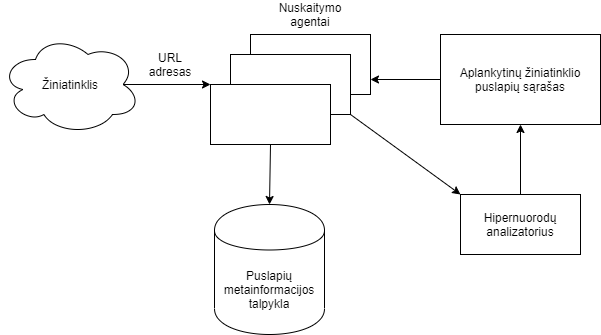
\includegraphics[scale=0.6]{img/Web_Crawler_Architecture.png}
\caption{Aukšto lygio saityno pežiūros roboto architektūra}
\label{fig:high_level_architecture}
\end{figure}


\subsection{Palyginimas su saityno duomenų rinkimo sistemomis}
Terminai \textbf{saityno žvalgymas} (angl. \textit{Web Crawling}) ir \textbf{saityno duomenų rinkimas} (angl. \textit{Web Scraping}) dažnai vartojami kaip sinonimai, nors jų reikšmės skiriasi. Siekiant įvesti aiškią skirtį ir apibrėžti darbe nagrinėjamo tipo sistemų funkcionalumo ribas, šiame skyriuje atliekamas terminų palyginimas. 

\subsubsection{Skirtumai}

Duomenų žvalgymas dažniausiai apima dideles saityno erdves -- vyksta tęstinis procesas, kurio metu siekiama identifikuoti puslapyje pasiekiamas hipernuorodas ir atlikti tų nuorodų tolimesnį žvalgymą. Tuo metu duomenų surinkimo sistema dažniausiai turi aiškų objektą ir jo struktūrą -- konkrečią svetainę ar duomenų bazę ir siekia išgauti tam tikrus dominančius duomenis. Galima teigti, jog saityno žvalgymo sistemos labiausiai suinteresuotos ryšių tarp puslapių nustatymui tam, kad būtų galima keliauti žiniatinkliu, o žiniatinklio duomenų surinkimo sistemų epicentre -- informacijos gavyba \cite{OxylabsScrapingVsCrawling}. \ref{tab:crawling_vs_scraping} lentelėje pateikta keletas esminių lyginamųjų charakteristikų tarp šių vartojamų terminų.

Nagrinėjami terminai skiriasi, tačiau yra itin susiję, nes saityno žvalgymas yra dažniausiai pirmasis informacijos gavybos etapas -- reikalingo turinio surinkimas. Žinoma, duomenų surinkimą galima atlikti be žvalgymo sistemų pagalbos, tačiau žvalgymo sistemos visada kartu naudoja duomenų surinkimo sistemas tam, kad atskirtų vertingą turinį nuo prastos reputacijos svetainės. \cite{OxylabsScrapingVsCrawling}

% Table generated by Excel2LaTeX from sheet 'crawling_vs_scraping'
\begin{table}[htbp]
  \centering
  \caption{Duomenų žvalgymo ir surinkimo sistemų palyginimas \cite{PromptCloudScrapingVsCrawling}}
    \begin{tabular}{|l|l|p{13.57em}|}
    \hline
    \textbf{Aspektas} & \textbf{Duomenų žvalgymas} & \textbf{Duomenų surinkimas} \bigstrut\\
    \hline
    Veikimo mastelis & Milžiniškas & Koncentruotas \bigstrut\\
    \hline
    Veikimo erdvė & Žiniatinklis & Žiniatinklis, duomenų bazė, serveris \bigstrut\\
    \hline
    Dublikatų aptikimas & Esminis veiksmas & Nebūtinas veiksmas \bigstrut\\
    \hline
    \multicolumn{1}{|p{12.285em}|}{Esminiai funkciniai komponentai} & Žvalgymo agentai & Žvalgymo agentai ir duomenų analizatoriai \bigstrut\\
    \hline
    Rankinio atlikimo galimybė & Negalima & Galima \bigstrut\\
    \hline
    Tikslas & Hipernuorodų aptikimas & Duomenų išgavimas \bigstrut\\
    \hline
    \end{tabular}%
  \label{tab:crawling_vs_scraping}%
\end{table}%

Šiame rašto darbe nagrinėjamos duomenų peržiūros robotų, dar vadinamų vorais (angl. \textit{Web Spider Bot}), sistemos, kurios keliauja saitynu naudojantis išgaunamomis HTML nuorodomis (angl. -- \textit{anchor tags}). Rašto darbe nėra aptariamas svetainės turinio duomenų apdorojimas, struktūrizuotos informacijos gavyba, nes tai nėra tokių sistemų atsakomybės sritys.

\subsection{Pagrindinės sistemos veikimo politikos}

Saityno peržvalgos roboto sistemų veikimo specifiką sudaro 4 pagrindinių naudojamų strategijų kombinacija. Kiekviena šių politikų yra atskira išsamiai aprašoma mokslinė saityno peržvalgos problema, reikalaujanti nuodugnios analizės, todėl šiuose punktuose šios politikos apžvelgiamos bendrais bruožais.

\subsubsection{Pasirinkimo politika}

Ši politika apibrėžia žvalgytinų puslapių prioritizavimo tvarką. Vienas didžiausių žiniatinklio žvalgymo iššūkių -- milžiniškas Interneto svetainių skaičius, kurio eksponentinis augimas išlieka iki šių dienų. Net patys efektyviausi saityno žvalgymo robotai neturi pakankamai resursų, jog galėtų padengti visas svetaines, todėl atsiranda efektyvaus prioritizavimo klausimas \cite{EffectiveWebCrawling}. Reikalinga efektyvi funkcija, kuri galėtų įvertinti žvalgytino puslapio kokybę dar prieš jį atsisiunčiant. Puslapio kokybę galima suprasti kaip kiekvieną iš šių faktorių:

\begin{itemize}
    \item Nuorodų, rodančių į puslapį, skaičius
    \item Puslapio semantinės temos atitikimas paieškos užklausai
    \item Puslapio semantikos atitikimas nuorodos tekstui
\end{itemize}

\subsubsubsection{Paieška į plotį}

Viena iš paprasčiausių žvalgymo politikų -- paieškos į plotį algoritmas, kurio principas pavaizduotas \ref{fig:bfs} paveikslėlyje. Atlikti eksperimentiniai žvalgymo tyrimai (aplankyta virš 300 mln. svetainių) parodė, jog paieškos į plotį strategija puikiai veikia surenkant aukštos kokybės puslapius žvalgymo pirmuose etapuose \cite{EffectiveWebCrawling}. Ši išvada grįsta nuomone, kad aukštesnės kokybės puslapiai turi daugiau nuorodų, vedančių į juos, todėl atrandami anskčiau \cite{EffectiveWebCrawling}.

\begin{figure}[htp!]
\centering
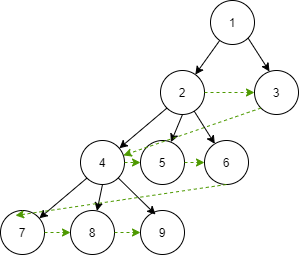
\includegraphics[scale=0.7]{img/BFS.png}
\caption{Paieškos į plotį grafas}
\label{fig:bfs}
\end{figure}

\subsubsubsection{PageRank algoritmo metrika}

Kitas būdas atlikti efektyvesnį žvalgymą -- kiekvienam lanktytinam puslapiui apskaičiuoti kokybės metriką ir lankyti aukštos metrikos vertės puslapius anskčiau. Viena iš tokių metrikų -- „Google“ patentuotas ir šios kompanijos pirmasis svetainių kokybės vertinimo algoritmas „PageRank“.

\begin{figure}[htp!]
\centering
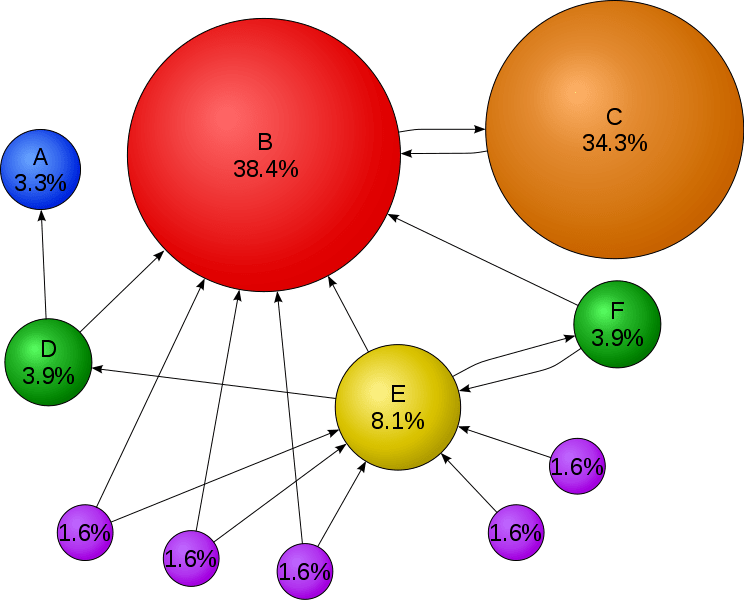
\includegraphics[scale=0.4]{img/pagerank.png}
\caption{„PageRank“ algoritmo principas \cite{PageRank}}
\label{fig:pagerank}
\end{figure}

Kaip galima pastebėti iš \ref{fig:pagerank} grafo, „PageRank“ algoritmas vertina nuorodų skaičių, kurios rodo į tam tikrą puslapį ir tų nuorodų puslapių kokybę. Matoma, jog B viršūnė turi aukštą autoritetą, nes į ją rodo daug mažų viršūnių, o C viršūnė -- nes į ją rodo viena aukšto autoriteto viršūnė.

\subsubsection{Etiško žvalgymo politika}

Saityno žvalgymo robotai veikia naudodami daug lygiagrečių žvalgymo procesų, kurie sugeneruoja didelius kiekius tinklo I/O srauto. Žvalgant konkretų žiniatinklio serverį, svarbu užtikrinti, jog priskirtas žvalgymo procesas nesutrikdytų sklandaus šio serverio darbo, t.y. nesukeltų netyčinės DoS\footnote{DoS - Denial of Service Attack} atakos \cite{EffectiveWebCrawling}. 

\subsubsubsection{REP protokolas}

Kaip dalinė etiško saityno žvalgymo užtikrinimo priemonė, buvo sukurtas \textit{Robots Exclusion Protocol} taisyklių rinkinys, kuriuo svetainių administratoriai gali nurodyti, kurias svetainės dalis jie leidžia robotams pasiekti, taip pat, koks galimas minimalus žvalgymo užklausų laiko intervalas. Pavyzdinis robots.txt failo turinys matomas \ref{fig:rep-example} paveikslėlyje.

\begin{figure}[htp!]
\centering
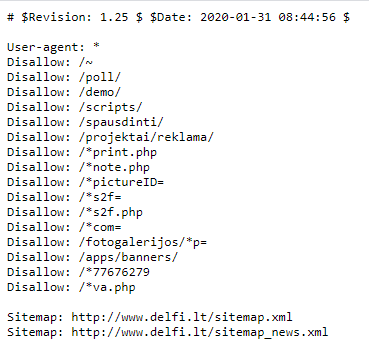
\includegraphics[scale=0.8]{img/rep_protocol.png}
\caption{delfi.lt robots.txt pavyzdys}
\label{fig:rep-example}
\end{figure}

\textit{User-agent} direktyva apibrėžia robotų pavadinimus, kuriems taikomas taisyklių rinkinys. Kiekvienas etiškas žvalgymo robotas kreipdamasis į žiniatinklio serverį identifikuoja save naudodamas šią HTTP antraštės reikšmę. Pavyzdžiui, „Googlebot“ sistema naudoja tokią šios HTTP antraštės reikšmę:
\begin{verbatim}
Mozilla/5.0 AppleWebKit/537.36 (KHTML, like Gecko; compatible; Googlebot/2.1; 
+http://www.google.com/bot.html) Chrome/W.X.Y.Z‡ Safari/537.36
\end{verbatim}
\textit{Disallow} direktyva nurodo, koks dokumentas ar byla negali būti pasiekiama tam tikram robotui. Taip pat gali būti naudojamas „*“ simbolis (\textit{angl. -- wildcard symbol}), nurodantis, jog taisyklių rinkinys turi būti taikomas bet kokiai reikšmei \cite{RobotsExclusionProtocol}.

Į oficialių standartą neįtraukta, bet dažnai sutinkama \textit{Crawl-delay} direktyva, kurią kiekvienas žvalgymo robotas gali interpretuoti skirtingai, dažniausiai tai būna laiko tarpas tarp skirtingų HTTP užklausų į serverį.

Akcentuotina, kad šis protokolas negarantuoja, jog robotas nežvalgys uždraustų direktorijų ar resursų, nes žiniatinklyje yra daugybė neetiškų žvalgymo sistemų, siekiančių blogų tikslų.

\subsubsubsection{Svetainės žvalgymo intervalai}

Ši roboto sistemos charakteristika yra svarbiausia etiško žvalgymo politikoje. Turi būti išlaikytas balansas tarp žvalgymo mandagumo (neapkraunamas žiniatinklio serveris) ir peržvalgos efektyvumo, nes didelės svetainės, turinčios šimtus tūkstančių puslapių, turi būti žvalgomos itin greitai \cite{EffectiveWebCrawling}.

\subsubsection{Pakartotinio apsilankymo politika}

Inkrementinio tipo žvalgymo robotai turi užtikrinti, jog sistemos puslapių indekso repozitorijoje turimos lokalios puslapių kopijos yra kiek galima naujesnės ir atitinkančios originalų resursą esamu laiku. \cite{EffectiveWebCrawling}

Šiam tikslui yra apibrėžtos dvi pagrindinės funkcijos, sutinkamos literatūroje, kurios kartu nusako puslapio pokyčio neaptikimo kainą.

\subsubsubsection{Šviežumo funkcija}

Ši funkcija nusako, ar lokali kopija atitinka originalų resursą duotuoju laiko momentu ir gali būti apibrėžiama taip:

\[F\: p(t) = \left\{\begin{matrix} 1, & p & puslapis & atitinka & laiko & momentu & t\\ 0 & kitu & atveju \end{matrix}\right.\]

\subsubsubsection{Amžiaus funkcija}

Ši funkcija nusako, kokio senumo turima lokali puslapio p kopija:

\[A\: p(t) = \left\{\begin{matrix} 0, & p & puslapis & nepakeistas & laiko & momentu & t\\ t & kitu & atveju \end{matrix}\right.\]

\textit{t} reikšmė šiuo atveju nusako puslapio modifikavimo laiką.

\subsubsubsection{Pakartotinio apsilankymo strategijos}

Pagal \cite{EffectiveWebCrawling} dažniausiai sutinkamos 2 pakaertotinio žvalgymo strategijos:

\begin{enumerate}
    \item Vieningoji strategija -- visi puslapiai pakartotiniai žvalgomi kas tą patį laiko intervalą
    \item Proporcinė strategija -- dažniau kintantys puslapiai žvalgomi dažniau
    \item Svarbos strategija -- svarbesni puslapiai (taikomos metrikos įvertinti, pvz.: „PageRank“) žvalgomi dažniau
\end{enumerate}

Ištirta, jog vieningoji strategija plačiajame žvalgyme efektyvesnė už proporcinę \cite{EffectiveWebCrawling}.

\subsection{Peržiūros robotų kategorijos}

Saityno peržiūros robotų sistemos skirstomas į skirtingas kategorijas pagal taikomas žvalgymo strategijas. Jos bendrai apžvelgiamos šiame poskyryje.

\subsubsection{Teminiai žvalgymo robotai}

Šio tipo (angl. -- \textit{Focused Web Crawlers}) saityno žvalgymo sistemos parsiunčia tik puslapius, atitinkačius specifinę semantinę temą \cite{CategoriesOfWebCrawlersAndOverview}. Puslapiai būna glaudžiai semantiškai susiję vienas su kitu. Tokios sistemos turi sugebėti įvertinti svetainės atitikimą apibrėžtai žvalgymo temai ir nuspręsti, kokiu būdu judėti nuorodų grafu pirmyn. Viena iš pasiūlytų idėjų kaip atpažinti resurso aitikimo žvalgymo roboto temai laipsnį -- HTML žymių (angl. -- \textit{anchor tag}) elemento tekso indeksas ir jo semantinė analizė \cite{AnchorTagsSemanticAnalysis}. Strategijos silpnybė -- svetainių administratoriai lengvai gali manipuliuoti tekstu į resursus, kurie neatitinka žvalgymo robot tematikos.


\subsubsection{Inkrementiniai žvalgymo robotai}

Tradicinės literatūroje aprašytos saityno žvalgymo sistemos periodiškai atnaujina savo turimą žiniatinklio dokumentų indeksą pakeisdamos senus dokumentus naujai parsiųstais \cite{CategoriesOfWebCrawlersAndOverview}. Inkrementiniai robotai savo turimą indeksą keičia analizuodami kiekvieno resurso pokyčio laipsnį (įvairūs semantiniai algorimtai, NPL\footnote{NLP - Natural Language Processing} algoritmai). Tokie robotai taip pat pakeičia mažiau svarbius puslapius į labiau svarbesnius, todėl išsprendžiama indeksuotų resursų naujumo ir aktualumo problema, taip pat taupoma žvalgymo roboto sistemos disko vieta, interneto srautas.

\subsubsection{Išskirstyti žvalgymo robotai}

Ši kategorija labiau apibrėžia žvalgymo roboto sistemos topologinę struktūrą -- sistema susideda iš centrinio serverio, kuris valdo daug išskirstytų agentų: jiems priskiria URL adresus ir liepia atlikti HTTP žvalgybą \cite{CategoriesOfWebCrawlersAndOverview}. Tokios kategorijos sistemos skirtos išgauti plačiam žiniatinklio resursų padengiamumui, šiomis dienomis efektyviam žvalgymui tokia struktūrizacija yra tiesiog privaloma. Taip pat tokios struktūros sistemos yra atsparios tinklo ar serverių darbo nesklandumams, nes pavieniams agentams nutraukus darbą, gali būti priskiriami kiti, nauji lygiagretūs procesai \cite{CategoriesOfWebCrawlersAndOverview}.

\subsubsection{Lygiagretūs žvalgymo robotai}

Kategorija apibrėžia sistemos loginę struktūrą -- agentai gali veikti kaip lygiagrečios gijos, atliekančios HTTP užklausas vienu metu. Ši strategija yra būtina efektyviam puslapių parsiuntimo greičiui per laiko vienetą pasiekti \cite{CategoriesOfWebCrawlersAndOverview}.
\section{Peržiūros roboto architektūros}

Šiame skyriuje analizuojamos mokslinėje literatūroje aprašytos saityno peržiūros robotų realizacijos -- pagrindiniai komponentai, jų funkcinės atsakomybės, charakteristikos, atliekama palyginamoji analizė tarp skirtingų aprašytų sistemų.

\subsection{Peržiūros roboto komponentai}

M.Najorc ir C. Olston mokslinė saityno peržiūros sistemų robotų (\cite{StanfWebCrawl}) formalizuoja anksčiau literatūroje aprašytas tokių sistemų dizaino specifikas. Joje nusakoma išskirstyto peržiūros roboto architektūra -- skirtingose mašinose egzistuojantys žvalgymo procesai, kiekvienas jų turintis keletą lygiagrečiai veikiančių agentų gijų, kurios atlieka kartotinius žvalgymo ciklo žingsius, kuriuose dalyvauja išskiriami pagrindiniai 8 struktūriniai sistemos komponentai.

\subsubsection{„Pasienis“}

„Pasienio“ duomenų struktūra (angl. -- \textit{URL Frontier}) saugo URL\footnote{URL - Uniform Resource Locator} adresų sąrašą, kurie bus aplankyti, iš šio sąrašo paduodamas adresas žvalgymo agento gijai pagal atitinkamas žvalgymo mandagumo (angl. -- \textit{Politeness}) ir prioritizavimo (angl. -- \textit{Priority}) politikas (\cite{StanfWebCrawl}. Tai viena iš pagrindinių žvalgymo roboto būsenos duomenų struktūrų. Jai keliami šie pagrindiniai funkcionalumo reikalavimai:
\begin{itemize}
    \item Pridėti URL adresą į sąrašą
    \item Nuskaityti URL adresą iš sąrašo
\end{itemize}

\subsubsection{HTTP parsiuntimo modulis}

Žvalgymo agentui gavus URL adresą iškviečiamas HTTP modulis, kuris pirmiausia kreipiasi į \textit{DNS adreso išaiškinimo} komponentą tam, jog būtų nustatytas URL resurso serverio vardo IP protokolo adresas \cite{StanfWebCrawl}. Šis veiksmas reikalingas tam, kad būtų minimizuotas HTTP užklausos atsakymo laikas (išvengiama DNS išaiškinimo užklausų į išorinius serverius).

\subsubsection{Saityno nuorodų ištraukiklis}

Šis komponentas (angl. -- \textit{Link Extractor}) nuskaito parsiųsto HTML dokumento turinį ir išgauna visas HTML nuorodas tiek į išorinius (angl. -- \textit{Offsite Links}), tiek į vidinius (\textit{In-site Links}) žiniatinklio serverio puslapius \cite{StanfWebCrawl}.

\subsubsection{Adresų skirstiklis}

Šis modulis (angl. -- \textit{URL Distributor}) atsakingas už išgautų nuorodų priskyrimą atitinkamiems žvalgymo procesams \cite{StanfWebCrawl}.

\subsubsection{Adresų filtras}

Komponentas, kuris filtruoja priskirtus URL adresus ir gali išmesti taisyklių neatitinkančias nuorodas (pvz.: puslapiai, įtraukti į juodąjį sąrašą) \cite{StanfWebCrawl}. Taisyklės gali būti specializuotos kiekvienam žvalgymui atskirai.

\subsubsection{Dublikatų šalintojas}

Roboto dalis, kuri atlieką testą, ar URL nuoroda dar nebuvo aplankyta peržiūros metu, pagrindiniai keliami funkcionamulo reikalavimai \cite{StanfWebCrawl}:
\begin{itemize}
    \item Pridėti URL adreso aplankymo indikatorių į sąrašą
    \item Atlikti URL priklausymo sąrašui testą
\end{itemize}

\subsubsection{Adresų prioritizuotojas}

Komponentas (angl. -- \textit{URL Prioritizer}), kuris kiekvienam URL adresui priskiria tam tikrą prioritetą pagal specializuotus saityno peržiūros roboto sistemos pasirinkimo politikos faktorius, tokius kaip nustatomas puslapio svarbos laipsnis ar puslapio keitimosi greičio faktorius \cite{StanfWebCrawl}.


\subsection{Peržiūros vykdymo ciklas}

Atsivelgus į 3.1 poskyrio struktūrinius komponentus pagal \cite{StanfWebCrawl} pasiūlytą schematinį dizainą, galima sudaryti veiklos diagramą, parodančią sistemos ciklinį funkcionavimą.

\begin{figure}[ht]
\centering
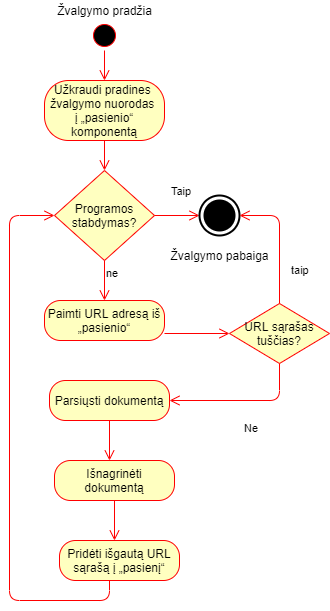
\includegraphics[scale=0.6]{img/Web_Crawler_Activity_Diagram.png}
\caption{Saityno žvalgymo roboto sistemos UML veiklos diagrama \cite{CategoriesOfWebCrawlersAndOverview}}
\label{fig:system_activity_diagram}
\end{figure}

\subsection{Literatūroje aprašytų robotų palyginamoji analizė}

Šiame skyriuje pristatomi esminiai inžineriniai peržiūros robotų architektūrų iššūkiai ir apžvelgiama keletas žinomiausių akademiniuose šaltiniuose aprašytų saityno peržiūros robotų architektūrų siekiant palyginti, kaip kiekvienas jų sprendžia minėtasias problemas.

\subsubsection{Peržiūros robotų archiktektūros iššūkiai}

Nors koncepcinis peržiūros sistemų algoritmas, aprašytas 1 skyriuje, yra labai paprastas, tokių sistemų problemos kyla sprendžiant išplėtimo iššūkius -- siekiant peržiūrėti milijardus svetainių per pagrįstai trumpą laiką ir išlaikyti peržiūrėtų svetainių naujausią galimą kopiją \cite{WCArchitectureMicrosoft}. Pagal \cite{WCArchitectureMicrosoft} apžvalgą, galima būtų iškelti šiuos pagrindinius peržiūros robotų architektūrų iššūkius:

\begin{itemize}
  \item Sugebėti vykdyti peržiūros procesą išskirstytai ir lygiagrečiai, tačiau vykdyti tai etiškai neapkraunant žiniatinklio serverio (etiško žvalgymo politika)
  \item Priklausymo sąrašui testas -- svarbu sugebėti efektyviai patikrinti (duomenų struktūros), ar URL adresas jau buvo peržiūrėtas
  \item Puslapio turinio dublikatų testas
  \item „Pasienio“ duomenų struktūra turi gebėti saugoti milijardus URL adresų
\end{itemize}

\subsubsection{„PolyBot“ sistema}

V. Shkapenyuk ir T. Suel aprašytas tinkle skirtinguose mazguose išskirstytas saityno peržiūros robotas, parašytas C++ ir Python programavimo kalbomis \cite{PolyBotArchitecture}.

Aprašyta architektūra (\ref{fig:polybot} schema) pasižymi peržiūros valdiklio komponentu, kuris gauna URL adresų užklausas ir paskirsto jas parsiuntimo komponentams \cite{PolyBotArchitecture}. Kiekvienas valdiklis gali komunikuoti daugiausiai su 8 parsiuntimo moduliais \cite{PolyBotArchitecture}. Peržiūros valdikliai tokioje architektūroje sukelia „butelio kaklelio“ efektą. Kitas apribojantis šios architektūros komponentas -- peržiūros programa (angl. -- \textit{Crawling Application}), kuri atsakinga už HTML dokumentų apdorojimą, peržiūros prioritizavimą ir žvalgytinų puslapių perdavimą valdikliui \cite{PolyBotArchitecture}. Kaip teigiama \cite{PolyBotArchitecture} šaltinyje, šis komponentas gali daugiausiai apdoroti 400 puslapių per sekundę.

\begin{figure}[htp!]
\hspace{-1cm}
\centering
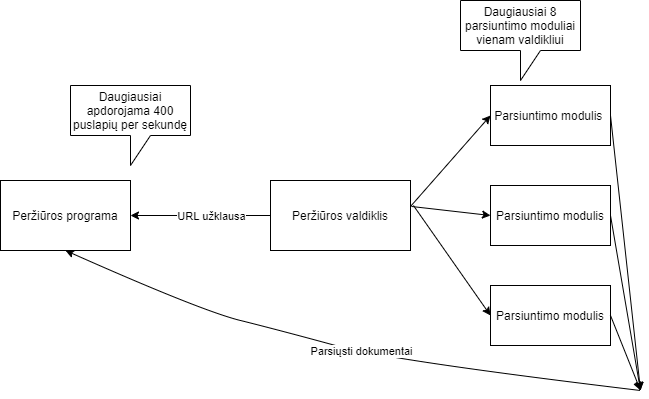
\includegraphics[scale=0.6]{img/plybot.png}
\caption{„Polybot“ peržiūros roboto architektūra}
\label{fig:polybot}
\end{figure}

\subsubsection{„Mercator“ sistema}

1999 m. išsamiai literatūroje autorių A.Heydon ir M.Najork aprašyta ir eksperimentiškai įvertinta išplečiama, paskirstyta saityno peržvalgos roboto sistemos architektūra. Ši sistema parašyta naudojantis Java programavimo kalba ir jos vykdomąja aplinka (angl. \textit{runtime environment}). Aprašyta sistema didžiąją dalį savo aprašomų duomenų struktūrų talpina disko atmintyje, taip pat nedideli buferiai saugomi operatyvioje atmintyje ir skirti pasiekti greitesnei duomenų prieigai (kešavimo mechanizmas) \cite{MercatorLiterature}.

\subsubsubsection{Žvalgymo agentai}

Sistemoje saityno žvalgymas vyksta naudojant žvalgymo procesų gijas (angl. \textit{worker threads}, kurios veikia lygiagrečiai ir įprastai sistemoje skaičiuojamos šimtais vienetų vienu metu \cite{MercatorLiterature}. Kiekviena gija atsakinga už puslapio atsiuntimą ir apdorojimą (nuorodų suradimą, suabsoliutinimą).

\subsubsubsection{Pagrindiniai sistemos komponentai}

Aprašomos sistemos išsamesnė schema pateikiama šio rašto darbo priede. Šioje dalyje trumpai apžvelgiamos kiekvieno komponento svarbiausios charakteristikos.


\subsubsubsection{„URL siena“}

Šis komponentas (angl. \textit{URL frontier}) saugo visų lankytinų URL adresų sąrašą, sudarytas iš nepriklausomų FIFO (angl. \textit{First-In-First-Out}) principu veikiančių eilių (angl. \textit{queues}), kurių kiekviena priskiriama atitinkam žvalgymo agentui. Taip pat, kai naujas URL adresas pridedamas į kurią nors eilę, konkreti eilė apsprendžiama pagal pridedamo adreso kanoninį vardą (angl. \textit{canonical host name}). Šie du principai įgyvendina žvalgymo roboto sistemos „mandagumo“ politiką -- užtikrinama, jog daugiausiai tik vienas žvalgymo agentas apdoros konkretų saityno serverį, todėl sistema neapkraus žvalgomo serverio resursų.

\vspace{1em}
\textbf{URL adresų saugojimas}
\vspace{1em}

Kadangi saugomas URL adresų sąrašas talpina šimtus milijonų įrašų, nagrinėjamoje sistemoje jie saugomi disko atmintyje, taip pat turimas 600 adresų buferis, saugomas operatyvioje atmintyje ir leidžiantis greičiau apdoroti nuorodas (išimti, idėti).

\subsubsubsection{„HTTP protokolo modulis“}

Peržvalgos robotų sistemos turi atsižvelgti į saityno serveriuose talpinamus \textit{robots.txt} failus, įgyvendinančius REP (angl. \textit{Robots Exclusion Protocol}) ir apibrėžiančius, kokie resursai pateiktame serveryje yra leistini žvalgyti. Aprašomos sistemos HTTP modulis saugo $2^18$ eilės serverio vardo-REP failo kešą.

\subsubsubsection{Įvesties srauto komponentas}


\subsubsection{„BUbiNG“ didelio masto žvalgymo sistemos architektūra}
\section{Dinaminių puslapių peržiūros problema}

Saityno peržvalgos robotų sistemų tradicinis modelis remiasi HTTP užklausomis į konkretų žiniatinklio serverį, kurį identifikuoja URL adresas. Taigi, tradicinės tokių sistemų implementacijos darydavo prielaidą, jog URL adresas unikaliai identifikuoja statinį turinį žiniatinklyje. Šis požiūris tapo nebetinkamas, kai W3C konsorciumas standartizavo AJAX\footnote{AJAX - Asynchronous JavaScript and XML} formatą asinchroninei žiniatinklio kliento komunikacijai su serveriu \cite{AJAXCrawlResearch}. Išplito dinaminiai puslapiai, kurie savo turinio dalis keičia asinchroniškai bendraudami su serveriu ir apsikeisdami informacija. Ši problema tapo itin aktuali su Vieno puslapio aplikacijų \footnote{SPA - Single Page Applications} ir jų kūrimo karkasų, tokių kaip React, Angular ar VueJS išpopuliarėjimu. Šiame skyriuje palyginamas tradicinis žiniatinklio resursų modelis su nauju, AJAX technologija grįstu modeliu, apžvelgiamos rinkoje taikomos praktikos naujo tipo žiniatinklio programų žvalgymui.

\subsection{Tradicinis žiniatinklio programos modelis}

Tradicinis žiniatinklio programos modelis remiasi sinchronine kliento-serverio komunikacija, kurioje klientas neturi jokios verslo logikos, visa puslapio žymėjimo ir stiliaus kodo sukonstravimo logika vyksta serverio pusėje. Tokiame modelyje saityno serveriai apkraunami tinklo užklausomis, nes norint pakeisti ar atnaujinti bet kokią puslapio dalį, reikalinga perkrauti visą puslapį iš naujo -- nusiųsti pakartotinę HTTP užklausą serveriui. Supaprastinta tokio modelio schema pateikiama \ref{fig:traditional_web_model} paveikslėlyje. 

\begin{figure}[htp!]
\centering
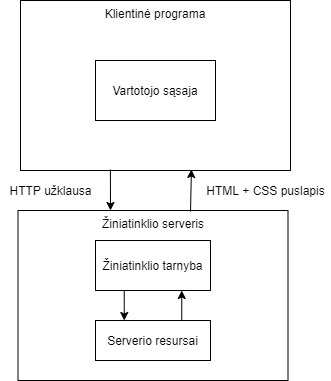
\includegraphics[scale=0.6]{img/Traditional_Web_Model.png}
\caption{Tradicinis žiniatinklio svetainės komunikacijos modelis \cite{AJAXCrawlResearch}}
\label{fig:traditional_web_model}
\end{figure}

Pagrindiniai tokio modelio trūkumai:
\begin{itemize}
    \item Visa kodo vykdymo logika atliekama serveryje
    \item Pakartotinis dublikuotų duomenų perdavimas
    \item Ganėtinai lėti serverio atsako laikai dėl pilno resurso užklausimo
\end{itemize}

\subsection{AJAX žiniatinklio programos modelis}

AJAX modelis taikomas naujo tipo vieno puslapio žiniatinklio svetainėse, kurių pagrindinis bruožas -- būsena kliento pusėje ir jos atnaujinimas dinamiškai reaguojant į kliento įvykius (angl. -- \textit{DOM Events}) ir siunčiant asinchronines AJAX užklausas į serverį. Detalesnė tokio modelio schema pateikiama \ref{fig:client_side|_rendering} paveikslėlyje.

\begin{figure}[htp!]
\centering
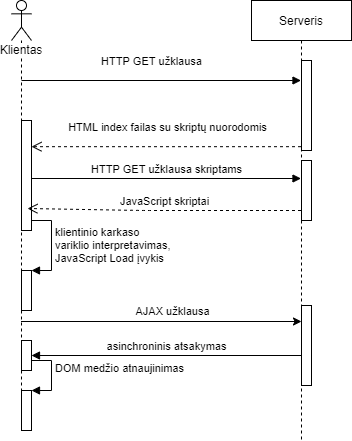
\includegraphics[scale=0.7]{img/csr.png}
\caption{Kliento pusės atvaizdavimas \cite{JavaScriptCrawl}}
\label{fig:csr}
\end{figure}

\subsubsection{AJAX modelio žvalgymo problema}

Tradiciniai žvalgymo robotai keliauja žiniatinklio grafu vykdydami HTTP GET užklausas, išgaudami nuorodas tiesiai iš serverio grąžinamo HTML kodo. Naujojo AJAX modelio svetainės reikalauja, jog svetainė būtų užkraunama pilnai, t.y. atsiunčiamas ir įvykdomas JavaScript kodas. Kitaip tariant, paieškos žvalgymo robotas turi elgtis panašiai kaip paprastas naršykle besinaudojantis žmogus \cite{JavaScriptCrawl}.

\subsubsubsection{„Googlebot“ taikoma praktika žvalgant AJAX svetaines}

„Googlebot“ žvalgymo robotas paiešką atlieka 3 etapais:

\begin{enumerate}
    \item Žvalgymas (angl. -- \textit{Crawling})
    \item Atvaizdavimas (angl. -- \textit{Rendering})
    \item Indeksavimas
\end{enumerate}

Atvaizdavimo etapas atliekamas būtent AJAX tipo dinaminėms svetainėms, kaip skelbiama „Google“, šiam procesui naudojama atvaizdavimo eilė, iš kurios agentai žinutes paima tuomet, kai atsilaisvina „Google“ žvalgymo infrastruktūros resursai. Tipiškai tai gali užtrukti nuo kelių minučių iki kelių savaičių. Šio modelio pagrindinė problema -- poreikis turėti efektyvią indikaciją, jog puslapis reikalauja Javascript atvaizdavimo ir jį reikia siųsti į atvaizdavmo eilę. Išsamesnė „Googlebot“ žvalgymo ir atvaizdavimo (angl. -- \textit{Rendering}) schema pavaizduota \ref{fig:googlebot_rendering} paveikslėlyje.

\begin{figure}[htp!]
\centering
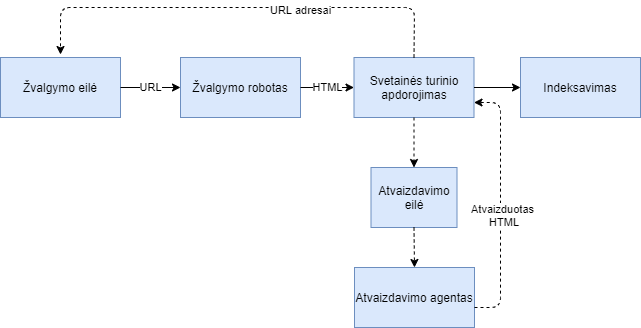
\includegraphics[scale=0.7]{img/Googlebot_rendering.png}
\caption{„Googlebot“ žvalgymo procesas \cite{GooglebotCrawling}}
\label{fig:googlebot_rendering}
\end{figure}

Pavaizduotoje schemoje atvaizdavimo procese yra naudojamas „Chromium“ naršyklės variklis be vartotojo sąsajos, kuris sugeba įvykdyti svetainės JavaScript kodą. Tiesa, „Google“ neatskleidžia, koks roboto svetainės užkrovimo maksimalus laukimo laikotarpis. Kaip teigiama, kol kas „Chromium“ variklis yra leidžiamas atskirai nuo bendrų „Google Chrome“ naršyklės išleidimų, todėl jo funkcionalumai ir palaikomos ECMAScript naujovės atsilieka, todėl atvaizdavimo metu „Googlebot“ gali nesuprasti naujausių svetainės sintaksės elementų. \cite{GooglebotCrawling}.

Šiame skyriuje pristatytos dinaminių svetainių atvaizdavimo schemos realizacija (technologijos ir priemonės) nagrinėjama praktinėje rašto darbo dalyje, 4 ir 5 skyriuose, kuriuose taip pat nurodoma, kokiu algoritmu įgyvendinamame prototipe priskiriama indikacija, jog svetainė reikalauja dinaminio Javascript atvaizdavimo.
\subsection{Reikalavimai prototipinei sistemai}
Šiame poskyryje pagal išnagrinėtą teorinę medžiagą apibrėžiami reikalavimai prototipinei sistemai.
\subsubsection{Funkciniai reikalavimai}
Žemiau, \ref{tab:functional_requirements} lentelėje pateikiami sudaryti prototipo funkcionalumo reikalavimai, atsižvelgiant į pirmame ir antrame skyriuose analizuotą peržiūros robotų literatūros teorinę medžiagą.

% Table generated by Excel2LaTeX from sheet 'Sheet1'
\begin{table}[htbp]
  \centering
  \caption{Funkciniai prototipo reikalavimai}
    \begin{tabular}{|l|p{23.785em}|}
    \hline
    \textbf{Numeris} & \multicolumn{1}{l|}{\textbf{Reikalavimo aprašymas}} \bigstrut\\
    \hline
    FR1   & Paduoti pradinį žvalgymo adresų sąrašą \bigstrut\\
    \hline
    FR2   & HTTP protokolo pagalba nuskaityti svetainės turinio kodą ir surasti visus saitus (angl. „hyperlinks“) \bigstrut\\
    \hline
    FR3   & Atlikti rekursyvų puslapių žvalgymą „į plotį“ grįstu algoritmu \bigstrut\\
    \hline
    FR4   & Sukelti rastus naujus saitus į žvalgytinų adresų sąrašo eilę \bigstrut\\
    \hline
    FR5   & Filtruoti žvalgytinus adresus pagal dominančius nuorodų kriterijus (plečiamumas) \bigstrut\\
    \hline
    FR6   & Atsižvelgti į „Robots Exclusion“ protokolą (robots.txt) žiniatinklio serveriuose \bigstrut\\
    \hline
    FR7   & Identifikuoti sistemą naudojantis User-Agent HTTP antraštės lauku \bigstrut\\
    \hline
    FR8   & Saugoti žvalgymo rezulatus svetainių indekso repozitorijoje \bigstrut\\
    \hline
    FR9   & Įgyvendinti mandagaus žvalgymo politiką: žiniatinklio serverio žvalgymo greitį nuspręsti iš HTTP atsako laiko, svetainės populiarumo metrikos \bigstrut\\
    \hline
    FR10  & Išgauti saitų nuorodas iš dinaminių Javascript atvaizdavimą naudojančių žiniatinklio svetainių \bigstrut\\
    \hline
    FR11  & Identifikuoti jau aplankytas nuorodas \bigstrut\\
    \hline
    \end{tabular}%
  \label{tab:functional_requirements}%
\end{table}%

\subsubsection{Nefunkciniai reikalavimai}
% Table generated by Excel2LaTeX from sheet 'Sheet1'
\begin{table}[htbp]
  \centering
  \caption{Nefunkciniai prototipo reikalavimai}
    \begin{tabular}{|l|p{23.785em}|}
    \hline
    \textbf{Numeris} & \multicolumn{1}{l|}{\textbf{Reikalavimo aprašymas}} \bigstrut\\
    \hline
    NFR1   & Naudoti tik debesų kompiuterijos viešų tiekėjų PaaS, SaaS, IaaS sprendimus \bigstrut\\
    \hline
    NFR2   & Dinamiškai koreguoti sistemos žvalgymo pajėgumus \bigstrut\\
    \hline
        NFR3   & Turi galioti beveik tiesinė priklausomybė tarp sistemos resursų ir žvalgymo pajėgumų \bigstrut\\
    \hline
            NFR4   & Žvalgyti bent 100 puslapių per sekundę greičiu (250 milijonų puslapių per mėnesį) \bigstrut\\
    \hline
    \end{tabular}%
  \label{tab:non_functional_requirements}%
\end{table}%

\section{Pasirinktos debesų kompiuterijos technologijos}

Šis skyrius žymi praktinės rašto darbo dalies pradžią, jame apžvelgiamos pasirinktos „Microsoft Azure“ debesų kompiuterijos tiekėjo paslaugos ir resursai argumentuojant pasirinkimo motyvus. „Azure“ platforma pasirinkta dėl autoriaus asmeninės patirties, tačiau rašto darbo autorius neabejoja dėl galimybės panašias paslaugas pasirinkti kitų tiekėjų, tokių kaip „Amazon AWS“ \footnote{AWS -- Amazon Web Services} ar „Google Cloud Platform“ platformose. \cite{MercedCloudBasedWebCrawler} moksliniame darbe, kuriuo šiame rašto darbe plačiai remiamasi kuriant peržiūros robotą, aprašyta sistema  buvo kurta pagal senąjį „Azure“ infrastruktūros modelį, kuris šiuo metu aktyviai nebepalaikomas, todėl įgyvendinant šį prototipą buvo pasitelkti naujesni „Azure“ debesų kompiuterijos tiekėjo įrankiai, kurie leistų užtikrinti analogišką aprašytos architektūros įgyvendinimą.

\subsection{Sistemos orchestravimas}

Įgyvendinant detalųjį architektūrinį saityno peržvalgos roboto sistemos dizainą ir renkantis iš technologijų, buvo pasirinkta „Microsoft Azure Service Fabric“ mikroservisų orchestravimo platforma, kuri apibrėžia ne tik sistemų klasterių valdymą ir išplėtimą, tačiau taip pat turi savo vykdomąją aplinką (angl. -- \textit{Service Fabric Runtime Environment}), kuri palaiko „Service Fabric“ programavimo modelius \cite{ServiceFabricTerminology}. Alternatyvi galimybė buvo rinktis „Azure Kubernetes Service“ orchestratoriaus paslaugą, tačiau „Service Fabric“ buvo pasirinktas dėl didelių vykdomosios aplinkos ir programavimo modelių galimybių, kurios suteikia daug abstrakcijos programuotojams -- leidžia orientuotis į verslo kodo rašymą paliekant infrastruktūrines surišimo problemas pačiai platformai.

\subsubsection{„Service Fabric“ infrastruktūra}

Šios platformos infrastruktūros konceptą apibrėžia 3 pagrindiniai komponentai \cite{ServiceFabricTerminology}:
\begin{itemize}
    \item Klasteris (angl. -- \textit{Cluster}) -- tinklu sujungtas išplečiamas rinkinys virtualių ar fizinių mašinų, kuriose diegiami „Service Fabric“ programų paketai, gali turėti kelis priskirtus mazgo tipus
    \item Mazgo tipas (angl. -- \textit{Node Type}) -- komponentas, kuris sujungia „Service Fabric“ klasterį su „Azure“ virtualių mašinų rinkiniu. Gali turėti ne daugiau nei vieną priskirtą virtualių mašinų rinkinį
    \item Virtualių mašinų išplėtimo rinkinys (angl. -- \textit{Virtual Machine Scale Set}) -- virtualių mašinų kolekcija, kurioje galima pridėti/trinti mašinas
    \item Mazgas (angl. -- \textit{Node}) -- virtuali arba fizinė mašina, kuri yra sudedamoji klasterio dalis, turi priskiriamą vardą
\end{itemize}

\ref{fig:sf_infrastructure} paveikslėlyje matomas infrastruktūros komponentų išsidėstymas. Vienas mazgo tipas visada būna pirminis, o kiti -- antriniai. Nerekomenduojama keisti pirminio mazgo tipo virtualių mašinų korekcijos virtualias mašinas jau paleidus klasterį, nes pakeitimas gali turėti neigiamos įtakos sklandžiam klasterio veikimui. Rašto darbe prototipas sudiegtas į vieno mazgo tipo klasterį, tai leido sutaupyti kaštų -- ši paslauga nerekomenduojama produkcinėms aplinoms, tačiau skirta testavimo tikslams.

\begin{figure}[htp!]
\centering
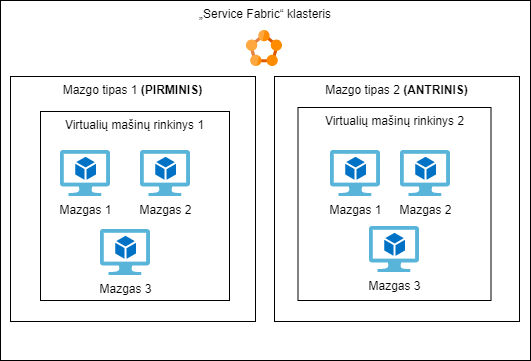
\includegraphics[scale=0.7]{img/SF_infrastructure.png}
\caption{„Service Fabric“ infrastruktūra \cite{ServiceFabricTerminology}}
\label{fig:sf_infrastructure}
\end{figure}

„Azure Service Fabric“ infrastruktūra palaiko tiek „Windows“, tiek „Linux“ operacines sistemas, rašto darbe naudojamas „Windows“ klasteris, kuris reikalauja daugiau minimalių sistemos resursų. Minimalūs rekomenduojami reikalavimai „Windows“ klasteriui yra šie:
\begin{itemize}
    \item 3,5 GB RAM operatyviosios atminties
    \item 50 GB SSD laikinos disko vietos
    \item 1 vienetas 2.4 GHz Intel Xeon vCPU procesorius
\end{itemize}
\subsubsection{„Service Fabric“ programavimo modelis}

„Service Fabric“ programavimo modelį sudaro šie pagrindiniai komponentai \cite{ServiceFabricTerminology}:

\begin{itemize}
    \item Programa (angl. -- \textit{Application}) -- rinkinys savarankiškų tarnybų (angl. -- \textit{Services}), kurios atlieka tam tikrą funkciją sistemoje
    \item Tarnyba (angl. -- \textit{Service}) -- tam tikros funkcijos atlikimo vienetas, mikroservisų architektūros vienetas
    \item Skaidinys (angl. -- \textit{Partition}) -- tarnybos duomenų skaidymo loginis vienetas, šiame rašto darbo prototipe nenaudojamas, todėl plačiau neaptariamas
    \item Kopija (angl. -- \textit{Replica}) -- duomenų kopijos, naudojamos tarnybose su būsena (angl. -- \textit{stateful services}), šio rašto darbo prototipo įgyvendinime nenaudojamos
\end{itemize}

\begin{figure}[htp!]
\centering
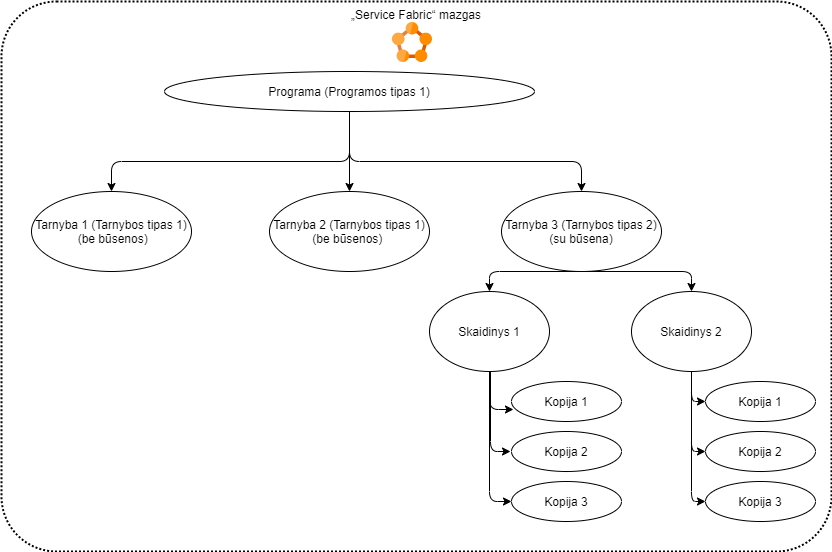
\includegraphics[scale=0.5]{img/SF_programming_model.png}
\caption{„Service Fabric“ programavimo modelis \cite{ServiceFabricTerminology}}
\label{fig:sf_programming_model}
\end{figure}

„Azure Service Fabric“ programavimo modelis apibrėžia 4 tipų tarnybas:
\begin{enumerate}
    \item Tarnybos be būsenos (angl. -- \textit{Stateless services}) -- tarnybos, kurios operatyvioje atmintyje nesaugo ir nenaudoja duomenų, visi duomenys išoriniai -- gali būti SQL duombazė ar NoSQL talpykla \cite{ServiceFabricTerminology}
    \item Tarnybos su būsena (angl. -- \textit{Stateful services}) -- tarnybos, kurios turi savo priskirtus duomenis ir būseną, kuri yra replikuojama tarp skirtingų mazgų klasteryje \cite{ServiceFabricTerminology}
    \item Išorinio kodo tarnybas (angl. -- \textit{Guest executables}) -- klateryje galima paleisti tarnybas, kurios vykdo išorinį vykdomąjį failą (.exe failą), kuris sukurtas visiškai kitomis programavimo kalbomis, nei vykdomoji „Service Fabric“ aplinka \cite{ServiceFabricTerminology}
    \item Konteinerių tarnybas (angl. -- \textit{Container services}) -- tarnybos paketą galima talpinti virtualiame konteineryje (pvz.: „Docker“), kuriame taip pat izoliuota „Service Fabric“ vykdomoji aplinka ir visos reikalingos priklausomos bibliotekos \cite{ServiceFabricTerminology} 
\end{enumerate}

Šiame rašto darbe peržiūros agentai įgyvendinti kaip tarnybos be būsenos, nes visa jiems reikalinga informacija saugoma arba eilėse, arba SQL/NoSQL duombazėse, todėl vidinės būsenos mechanizmai, kuriuos siūlo „Service Fabric“ modelis, nereikalingi.

\subsection{Virtualių mašinų rinkiniai}

„Service Fabric“ klasteris turi priskiriamus vieną arba daugiau virtualių mašinų rinkinius (angl. -- \textit{„Virtual Machine Scale Sets“}), kurie leidžia logiškai grupuoti daug virtualių mašinų, kurias galima valdyti centralizuotai -- diegti atnaujinimus, keisti konfigūracija. \cite{VirtualMachineScaleSets}. Visos virtualios mašinos rinkinyje yra sukuriamos iš bendro operacinės sistemos atvaizdžio (angl. -- \textit{OS image}). \cite{VirtualMachineScaleSets}.

Kuriant virtualių mašinų išplėtimo rinkinį, automatiškai sukuriamas ir apkrovos išlyginimo (angl. -- \textit{load balancing}) resursas, kuris leidžia reaguoti į virtualių mašinų apkrovų duomenis ir tolygiai paskirstyti srautą. \cite{VirtualMachineScaleSets}. Taip pat sukuriamas virtualus tinklas, kuris leidžia rinkinyje esančioms virtualioms mašinoms bendrauti vienai su kita.

Įgyvendinant šio rašto darbo prototipą naudojamas klasteris su vienu virtualių mašinų išplėtimo rinkiniu, kuriame sudiegta viena virtuali mašina.

\pagebreak

\subsection{Eilių mechanizmas}

Įgyvendinant išskaidytą peržvalgos robotą, asinchroninę komunikaciją tarp atskirų sistemos komponentų užtikrina eilių mechanizmas, veikiantis FIFO\footnote{First-In-First-Out} principu. „Azure“ paslaugų modelis siūlo 2 skirtingus eilių sprendimus:
\begin{itemize}
    \item „Service Bus Queues“ -- „Azure Storage“ paslaugų infrastruktūros dalis, paprasta REST programinė sąsaja \cite{QueuesStorageVsServiceBus}
    \item „Storage Queues“ -- „Azure messaging“ infrastruktūros dalis, specializuotai skirta sistemų integracijos šablonų įgyvendinimui (pvz.: -- „publish-subscribe“) modelis \cite{QueuesStorageVsServiceBus}
\end{itemize}

Platesnis šių sprendimų palyginimas matomas lentelėje.

% Table generated by Excel2LaTeX from sheet 'crawling_vs_scraping'
\begin{table}[htbp]
  \centering
  \caption{„Storage Queues“ ir „Service Bus Queues“ palyginimas \cite{QueuesStorageVsServiceBus}}
    \begin{tabular}{|l|l|l|}
    \hline
    \textbf{Aspektas} & \textbf{„Azure Storage Queues“} & \textbf{„Azure Service Bus Queues“} \bigstrut\\
    \hline
    Atsiradimo laikas & Atsirado anksčiau & Pristatyta vėliau, 2014 metais \\
    \hline
    Eilės talpa & 1 TB ir daugiau & <= 80GB \\
    \hline
    FIFO užtikrinimas & Negarantuotas & Garantuotas \\
    \hline
    „Long-polling“ palaikymas & Nepalaikoma & Palaikoma \\
    \hline
    „AMQP 1.0“ standartas & Nepalaikomas & Palaikomas \\
    \hline
    Automatinis „dead-letter“ mechanizmas & Nepalaikomas & Palaikomas \\
    \hline
    Eilių skaičius & Neribojamas & 10000 \\
    \hline
    \end{tabular}%
  \label{tab:agent_registry_table}%
\end{table}%

Įgyvendinant prototipą rašto darbo autoriaus sprendimu pasirinkta „Azure Service Bus Queues“ technologija dėl šių esminių priežasčių:

\begin{enumerate}
    \item Palaikoma „long-polling“ technologija -- kuriant „Service Fabric“ tarnybas ir jų klausytojus (angl. -- \textit{service listeners}) nenorėta cikle naudoti HTTP „polling“ metodo, kuris lemtų sudėtingesnės kodo infrastruktūros poreikį
    \item FIFO palaikymas -- norima, kad pirmiau aptikti puslapiai būtų atitinkamai žvalgomi greičiau
    \item Rasta biblioteka, kuri užtikrino „Service Fabric“ ir „Service Bus“ paslaugų integraciją be papildomo kodo rašymo\footnote{Service Fabric Service Bus -- https://github.com/loekd/ServiceFabric.ServiceBus}
\end{enumerate}

\subsubsection{Pasirinktos technologijos rizikos}

\cite{MercedCloudBasedWebCrawler} siūlytoje architektūroje buvo naudojama „Azure Storage Queues“ paslauga, pagrindinės rizikos, kurios gali kilti naudojant rašto darbo autoriaus pasirinktą technologiją yra susijusios su apribotu plečiamumu, nes „Service Bus“ nepalaiko daugiau nei 10000 eilių, o šiame roboto prototipe kiekvienas domenas turi dinamiškai sukuriamą agento eilę. Taip pat apribotas eilės dydis (80GB), nes platus žvalgymas apima dešimtis milijonų puslapių.

\subsection{Reliacinė duombazė}

Vienas iš prototipo komponentų -- agentų registras -- realizuotas panaudojant griežtą schemą palaikančios „Microsoft SQL Server“ reliacinės duomenų bazės atitikmenį „Azure“ platformoje, kuris veikia PaaS\footnote{Platform-as-a-service} principu -- „Azure SQL“ duomenų bazės serverį. Ši debesų kompiuterijos paslauga leidžia kontroliuoti ugniasienės nustatymus, kad tik tam tikrų IP adresų klientai galėtų komunikuoti su duomenų baze, todėl įgyvendinant prototipą, virtualių mašinų kolekcijos virtualus tinklas buvo pridėtas kaip SQL duomenų bazės ugniasienės taisyklė. Platforma taip pat palaiko automatinį resursų išplečiamumą, kuris gali būti vykdomas reaguojant į naudojimo apkrovų statistiką.

\subsubsection{Duombazės pajėgumo metrika}

Kuriant „Azure SQL“ serverį svarbu atsižvelgti, kokio galingumo duombazės serverio sistemai reikia. Kadangi ši paslauga veikia PaaS principu, duombazės serverio pajėgumas nėra nustatomas tradicine procesoriaus branduolių, operatyviosios atminties ir disko talpos kombinacija. Vietoje to naudojama abstraktesnė metrika, pavadinimu „Data Trancation Unit“ (toliau -- DTU) \cite{DTUMetric}.

DTU apibrėžimas pagal „Microsoft“ dokumentaciją -- maišyta procesoriaus, operatyviosios atminties, duomenų ir tranzakcijų įrašų I/O skaičiaus metrika. \cite{DTUMetric} Dvigubinant DTU skaičių atitikamai dvigubinamas duomenų bazei priskiriamų resursų pajėgumas.

\subsection{NoSQL saugykla}

Pastovus aplankytų URL adresų sąrašas, taip pat svetainių Javascript atvaizdavimo analizavimo kontrolinės sumos saugomos „Azure Table Storage“ NoSQL duomenų bazėje. Ši paslauga yra „Key-value“ tipo NoSQL duombazės tipo. 

Tokio tipo duomenų bazės yra tam tikra prasme maišos lentelės (angl. -- \textit{hash tables}) ir pasižymi \cite{KeyValueStores}:
\begin{itemize}
    \item Itin greitos užklausos pagal rakto reikšmę (ieškoti pagal reikšmę nėra efektyvu, lyginant su reliacinėmis duomenų bazėmis ir jų WHERE sakinių konstruktais)
    \item Nėra duomenų bazės schemos, todėl lengva prisitaikyti prie evoliucionuojančių sistemų ir duomenų
    \item Lengvą išplėsti tokios duomenų bazės talpą pagal poreikius, nes duomenys paskirstomi skirtinguose fiziniuose mazguose, sujungtuose tinklu
    \item Nepalaiko sudėtingų paieškos operacijų, reikalaujančių duomenų apjungimo, išorinių raktų ar duombazės procedūrų
\end{itemize}

\pagebreak

\subsubsection{„Azure Storage Table“ modelis}

Šios paslaugos esmę apibrėžia 4 pagrindiniai elementai \cite{TableStorageModel}:
\begin{itemize}
    \item \textit{„Storage“ paskyra} -- unikalus resurso savininko indentifikavimo ir autorizavimo mechanizmas
    \item \textit{Lentelė} -- paskyroje esantis obektų rinkinys, neturintis griežtos atributų schemos
    \item \textit{Esybė} -- atributų rinkinys, panašus į reliacinių duomenų bazių eilutę
    \item \textit{Atributas} -- (angl. -- \textit{properties}) rakto-reikšmės pora, nusakanti esybės konkretų požymį
\end{itemize}

Šių esybių sąryšis pavaizduotas \ref{fig:storage_table_model} paveikslėlyje:

\begin{figure}[htp!]
\hspace{-1cm}
\centering
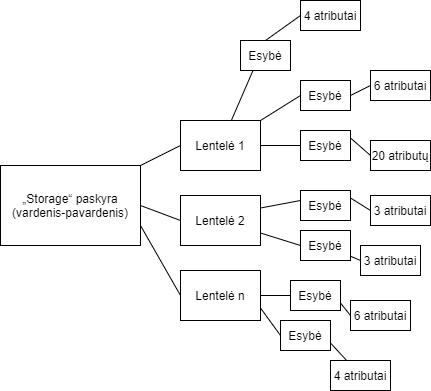
\includegraphics[scale=0.5]{img/Storage_modelis.png}
\caption{„Storage Table“ modelis}
\label{fig:storage_table_model}
\end{figure}

Aprašytos paslaugos modelyje esybė palaiko daugiausiai iki 255 atributų, iš kurių 3 yra sisteminiai ir privalomi: \cite{TableStorageModel}

\begin{itemize}
    \item \textit{PartitionKey} -- pirmoji sudėtinė pirminio rakto dalis, skaidinys, kuris leidžia skaidyti saugyklos duomenis topologiškai skirtinguose mazguose ir lemia didelį tokių duomenų bazių išplečiamumą
    \item \textit{RowKey} -- antroji sudėtinė pirminio rakto dalis, turi būti unikali kiekviename skaidinyje
    \item \textit{Timestamp} -- paskutinė esybės koregavimo data ir laikas
\end{itemize}

\begin{figure}[htp!]
\hspace{-1cm}
\centering
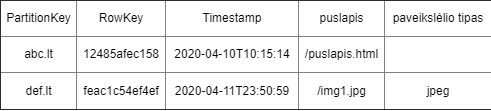
\includegraphics[scale=0.7]{img/Storage_table.png}
\caption{„Storage Table“ lentelės struktūra \cite{TableStorageModel}}
\label{fig:storage_table_structure}
\end{figure}

Kaip matome iš \ref{fig:storage_table_structure} lentelės, esybių atributų skaičius lentelėje gali skirtis, nes nėra apibrėžtos schemos.
\section{Prototipo realizacija}

Šis skyrius aprašo praktinę rašto darbo pusę -- debesų kompiuterijos technologijomis grįstos saityno peržiūros roboto realizacijos sprendimus. Architektūra ir naudojami įrankiai parinkti pagal 4 skyriuje apibrėžtus sistemos reikalavimus.

\subsection{Sistemos panaudojamumas}

Įgyvendinant prototipo architektūrą pagal 4 skyriuje išsikeltus reikalavimus, apibrėžtos pagrindinės veiklos, kurios sudaro sistemos funkcionalumą, jos matomos \ref{fig:use_case_diagram} paveikslėlyje pavaizduotoje UML panaudojamumo diagramoje.

\begin{figure}[htp!]
\centering
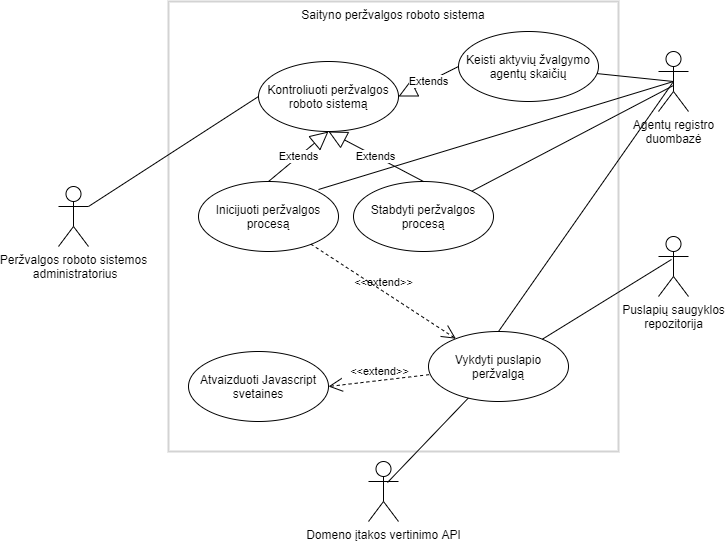
\includegraphics[scale=0.6]{img/Use_case_diagram.png}
\caption{UML žvalgymo roboto sistemos prototipo panaudojamumo diagrama}
\label{fig:use_case_diagram}
\end{figure}

Svarbu paminėti keletą aiškinamųjų aspektų apie \ref{fig:use_case_diagram} diagramoje pavaizduotas veiklas ir aktorius.


\textbf{Peržiūros roboto administratorius} -- klientinė programa, kontroliuojanti žvalgymo procesą. Klientas gali būti įvairių formų: komandinės eilutės programa, žiniatinklio, darbalaukio programa. Prototipo realizacijoje klientinė programa imituojama naudojantis \textit{„Service Bus Explorer“\footnote{https://github.com/paolosalvatori/ServiceBusExplorer}} įrankiu ir rankiniu būdu siunčiant žinutes į sistemos žvalgymo kontroliavimo eilę.

\textbf{Domeno įtakos vertinimo API} -- išorinis tarnybos serveris, kuris sugeba skalėje nuo 1 iki 100 įvertinti konkretaus domeno autoritetą, kuris reikalingas žvalgymo prioritizavimui. Prototipo įgyvendinimo metu naudota \textit{openrank.io\footnote{https://openrank.io/}} API paslauga, suteikianti 10000 nemokamų užklausų per 24 valandas. Akcentuotina, kad ši išorinė sistema nėra privaloma -- darbe pasirinkta etiško žvalgymo politika atsižvelgia į šią metriką siekiant nustatyti populiaresnes svetaines, kurias galima žvalgyti greičiau.

\textbf{Atvaizduoti Javascript svetaines} -- šis panaudojamumo atvejis yra vykdomas kaip atskira veikla po peržvalgos proceso, jei konkretus puslapis pasižymi dinaminės svetainės, kuri turinį generuoja klientinėje pusėje, savybėmis.

\subsubsection{Panaudojamumo atvejų paaiškinimai}
\ref{tab:use_case_table} lentelėje pateikti \ref{fig:use_case_diagram} diagramoje pavaizduotų panaudojamumo atvejų identifikatoriai ir detalesnis paaiškinimas:

% Table generated by Excel2LaTeX from sheet 'crawling_vs_scraping'
\begin{table}[ht]
  \centering
  \caption{Panaudojamumo atvejų paaiškinimai}
    \begin{tabular}{|p{2em}|p{13em}|p{20em}|}
    \hline
    \textbf{Id} & \textbf{Pavadinimas} & \textbf{Aprašymas} \bigstrut\\
    \hline
    U1.1 & Inicijuoti peržiūros procesą & Perkelti pradinį peržiūros URL adresų sąrašą į peržiūros eilę prieš tai patikrinti, ar URL adresai dar neperžiūrėti, ir sukurti pirmąjį peržiūros agentą, jam priskirti domeno vardo zoną \\
    \hline
    U1.2 & Stabdyti peržiūros procesą & Panaikinti visus aktyvius peržiūros robotus ir jų peržiūros eiles  \\
    \hline
    U1.3 & Keisti aktyvių peržiūros agentų skaičių & Padidinti arba pamažinti maksimalų leistiną peržiūros ir Javascript atvaizdavimo agentų kiekį sistemoje \\
    \hline
    U2 & Rekursyviai vykdyti puslapio peržiūrą & Aplankyti URL adresu nurodytą svetainę, išnagrinėti jos HTML turinį ir išgauti visas nuorodas, patikrinti, ar jos dar neperžiūrėtos, perduoti jas atitinkam peržiūros robotui  \\
    \hline
    U2.1 & Įvertinti, ar puslapis vykdo klientinį Javascript atvaizdavimą & Nustatyti, ar HTML dokumentas naudoja Javascript bibliotekas, kurios naudojamos klientinio atvaizdavimo vieno puslapio žiniatinklio programose, jei taip -- nusiųsti tokį URL adresą į Javascript atvaizdavimo eilę  \\
    \hline
    U2.2 & Įvertinti etiškos puslapio peržiūros laiko intervalą & Atsižvelgti į HTTP užklausos serverio atsakymo laiką, domeno populiarumą, robots.txt nurodytą leistiną peržiūros intervalą \\
    \hline
    U2.3 & Atvaizduoti Javascript svetaines & Naudojant Javascript variklį atvaizduoti pilną HTML turinį svetainėms, kurios naudoja klientinio atvaizdavimo bibliotekas \\
    \hline
    \end{tabular}%
  \label{tab:use_case_table}%
\end{table}%

\subsubsection{Atsekamumo matrica}

\ref{tab:requirements_use_case_traceability_matrix} lentelėje pateikta funkcinių, nefunkcinių reikalavimų ir nurodytų panaudojamumo atvejų atsekamumo matrica siekiant nurodyti, jog visi apibrėžti reikalavimai yra padengiami įgyvendinant peržiūros roboto prototipą.

% Table generated by Excel2LaTeX from sheet 'Sheet1'
\begin{table}[ht]
  \centering
  \caption{Reikalavimų ir panaudojamumo atvejų atsekamumo matrica}
    \begin{tabular}{|l|r|r|r|r|r|r|r|}
    \hline
          & \multicolumn{1}{l|}{\textbf{U1.1}} & \multicolumn{1}{l|}{\textbf{U1.2}} & \multicolumn{1}{l|}{\textbf{U1.3}} & \multicolumn{1}{l|}{\textbf{U2}} & \multicolumn{1}{l|}{\textbf{U2.1}} & \multicolumn{1}{l|}{\textbf{U2.2}} & \multicolumn{1}{l|}{\textbf{U2.3}} \bigstrut\\
    \hline
    \textbf{FR1} & \multicolumn{1}{l|}{\textbf{X}} &       &       &       &       &       &  \bigstrut\\
    \hline
    \textbf{FR2} &       &       &       & \multicolumn{1}{l|}{\textbf{X}} &       &       &  \bigstrut\\
    \hline
    \textbf{FR3} &       &       &       & \multicolumn{1}{l|}{\textbf{X}} &       &       &  \bigstrut\\
    \hline
    \textbf{FR4} & \multicolumn{1}{l|}{\textbf{X}} &       &       & \multicolumn{1}{l|}{\textbf{X}} &       &       &  \bigstrut\\
    \hline
    \textbf{FR5} &       &       &       & \multicolumn{1}{l|}{\textbf{X}} &       &       &  \bigstrut\\
    \hline
    \textbf{FR6} &       &       &       & \multicolumn{1}{l|}{\textbf{X}} &       & \multicolumn{1}{l|}{\textbf{X}} &  \bigstrut\\
    \hline
    \textbf{FR7} &       &       &       & \multicolumn{1}{l|}{\textbf{X}} &       &       & \multicolumn{1}{l|}{\textbf{X}} \bigstrut\\
    \hline
    \textbf{FR8} &       &       &       & \multicolumn{1}{l|}{\textbf{X}} &       &       & \multicolumn{1}{l|}{\textbf{X}} \bigstrut\\
    \hline
    \textbf{FR9} &       &       &       &       &       & \multicolumn{1}{l|}{\textbf{X}} &  \bigstrut\\
    \hline
    \textbf{FR10} &       &       & \multicolumn{1}{l|}{\textbf{X}} &       &       &       &  \bigstrut\\
    \hline
    \textbf{FR11} &       &       &       &       & \multicolumn{1}{l|}{\textbf{X}} &       & \multicolumn{1}{l|}{\textbf{X}} \bigstrut\\
    \hline
    \textbf{FR12} & \multicolumn{1}{l|}{\textbf{X}} &       &       & \multicolumn{1}{l|}{\textbf{X}} &       &       & \multicolumn{1}{l|}{\textbf{X}} \bigstrut\\
    \hline
    \textbf{NFR1} & \multicolumn{1}{l|}{\textbf{X}} & \multicolumn{1}{l|}{\textbf{X}} & \multicolumn{1}{l|}{\textbf{X}} & \multicolumn{1}{l|}{\textbf{X}} & \multicolumn{1}{l|}{\textbf{X}} & \multicolumn{1}{l|}{\textbf{X}} & \multicolumn{1}{l|}{\textbf{X}} \bigstrut\\
    \hline
    \textbf{NFR2} &       &       & \multicolumn{1}{l|}{\textbf{X}} &       &       &       &  \bigstrut\\
    \hline
    \textbf{NFR3} &       &       &       &       &       &       &  \bigstrut\\
    \hline
    \end{tabular}%
  \label{tab:requirements_use_case_traceability_matrix}%
\end{table}%


\subsection{Naudojama architektūra}

Prototipas rengiamas plačiai remiantis Kalifornijos Mersedo universiteto mokslininkų literatūrine medžiaga apie debesų kompiuterijos išskirstyto saityno žvalgymo roboto sistemą ir jos architektūrą, dizaino principus \cite{MercedCloudBasedWebCrawler}. Atsižvelgiant į darbo rašymo metus ir patobulėjusias debesų kompiuterijos tiekėjų siūlomas technologijas, pasiūlyta architektūra realizuojama pritaikius specifinius pokyčius pakeičiant realizacijos įrankius ir platformas. Šiame poskyryje aprašomi pasiūlytos architektūros pagrindiniai komponentai, pavaizduoti \ref{fig:mersed_architecture} diagramoje ir jų funkcinės atsakomybės.

\pagebreak

\begin{figure}[ht]
\centering
\includegraphics[scale=0.6]{img/Mersed_architektūra.png}
\caption{Mersedo universiteto mokslininkų pasiūlyta saityno peržiūros roboto architektūra \cite{MercedCloudBasedWebCrawler}}
\label{fig:mersed_architecture}
\end{figure}


\subsubsection{Centrinis žvalgymo variklis}
 
 Tai pagrindinis sistemos struktūrinis komponentas, kuris inicijuoja visą žvalgymo procesą ir kuria/naikina žvalgymo agentus. Pagrindiniai šio komponento veikimo etapai:
 \begin{enumerate}
     \item Inicializacija
     \begin{enumerate}
         \item Paimami pradiniai URL adresai iš žvalgymo adresų sąrašo
         \item Adresai sudedami į „Azure“ eilę prieš tai patikrinant, ar kiekvienas URL adresas dar nebuvo žvalgytas ( naudojamas \textit{„Azure NoSQL Table Storage“})
         \item Sukuriamas pirmasis žvalgymo agentas, jam priskiriama jo žvalgymo zona (svetainės serverio vardas)
     \end{enumerate}
     \item Ciklinis žvalgymo procesas
     \begin{enumerate}
         \item Iš žvalgymo eilės paimamas URL adresas
         \item Patikrinama, ar esamam URL adresui egzistuoja aktyvus agentas (SQL Agentų registro duombazė)
         \item Jei agentas egzistuoja, URL adresas ignoruojamas, nes priskirtas agentas jį apdoros
         \item Jei aktyvaus agento nėra, paskaičiavus aktyvių agentų skaičių A\textsubscript{aktyvūs} tikrinamas maksimalus leistinas agentų skaičius A\textsubscript{max} > A\textsubscript{aktyvūs}, jei sąlyga patenkinta, bandoma sukurti naują agentą ir jam priskirti URL adreso vardo zoną. Kitu atveju laukiama, kol sąlyga bus patenkinta (agentai baigs savo darbą).
         \item Kartojama nuo pirmo žingsnio
     \end{enumerate}
 \end{enumerate}
 
 \subsubsection{Žvalgymo agentas}

Šis komponentas iš žvalgymo eilės ima URL adresą, jei adreso vardo sritis sutampa su agentui priskirtu aptarnavimo vardo adresu, jis inicijuoja HTTP užklausą į nurodytą žiniatinklio serverį, parsiunčia HTML turinį, išgauna visas jame esančias nuorodas, kiekvienai jų patikrina, ar nuoroda dar neregistruota indeksų repozitorijoje ir atitinkamai perduoda aktyviam žvalgymo agentui, kurio zona sutampa su URL adreso vardo zona \cite{MercedCloudBasedWebCrawler}. Agentai užtikrina išskirstytos sistemos veikimo principą, juos galima dinamiškai pridėti, šalinti. Apibrėžtoje architektūroje nėra centrinio komunikacijos komponento, kuris deleguotų žvalgymo darbus agentams.

 \subsubsection{Agentų registras}
 
 Tai SQL duombazė, kurioje registruojami visi aktyvūs agentai, taip pat jie periodiškai išregistruojami aptikus, jog agentas kurį laiką nebuvo aktyvus. Šis komponentas yra bendras, todėl rašto darbo paskutiniame skyriuje, atliekant tyrimą, bus analizuojama, ar jis negali lemti „butelio kaklelio“ efekto.
 
 \subsubsection{„Azure“ žvalgymo eilė}
 
 Tai komponentas, kuris saityno žvalgymo sistemų literatūroje minimas kaip „žvalgymo pasienio“ (angl. -- \textit{Crawling Frontier}) komponentas, kuriame laikinai kaupiami žvalgytinų puslapių URL adresai \cite{EffectiveWebCrawling}. Žvalgymo agentai ir Centrinis žvalgymo variklis klausosi šios eilės žinučių ir jas apdoroja. Tai dar vienas bendrinis sistemos komponentas, todėl eksperimento metu taip pat bus stebimas jo veikimo pralaidumas. \cite{MercedCloudBasedWebCrawler} moksliniame darbe jau buvo atliktas šio komponento tyrimas ir įsitikinta, kad didinant žinučių kiekio apkrovą, komponento pralaidumas išlieka gana patovus. Naudota „Azure Storage Queues“ eilių paslauga. Šio rašto darbo tyrime naudojama „Azure Service Bus“ eilių infrastruktūra, todėl taip pat pakartotinai bus stebimas komponento veikimo pralaidumas.
 
 \subsubsection{„Azure“ NoSQL indeksų repozitorija}

Tai NoSQL rakto-reikšmės (angl. -- \textit{Key-Value}) tipo saugykla, kurioje agentai registruoja identifikuotus svetainių URL adresus, taip pat keičia tų adresų žvalgymo statusą, aptiktų URL nuorodų paminėjimų skaičių (angl. -- \textit{hit count}) \cite{MercedCloudBasedWebCrawler}.

\subsubsection{„Azure“ didelių objektų saugykla}

Šis komponentas aprašytoje architektūroje atsakingas už didelių multimedijos failų saugojimą -- nuotraukų, vaizdo įrašų, PDF dokumentų ir kitų žiniatinklio resursų, kurie nėra HTML dokumentai \cite{MercedCloudBasedWebCrawler}. Pasižymi tuo, jog gali talpinti didelius kiekius duomenų.

\subsubsection{Svetainės turinio analizatorius ir dublikatų aptikimas}

Vienas iš minimų sistemos komponentų -- svetainės turinio analizatorius -- semantiškai apdoroja nuskaitytą HTML dokumento turinį siekdamas nustatyti puslapio tematiką, pagrindinius raktinius žodžius, taip pat identifikuoti pasikartojančio, dublikuoto turinio svetaines. Šio prototipo įgyvendinimo ribose nebuvo numatytas semantinis svetainės turinio analizavimas, todėl plačiau šie komponentai aptariami nebus. Prototipo įgyvendinimo ribose nuamtytas tik URL adresų dublikatų aptikimas siekiant išvengti bereikalingos pakartotinės resurso žvalgymo naštos.

\subsection{Struktūrinė prototipo schema}

Šiame poskyryje aprašoma koreguota \cite{MercedCloudBasedWebCrawler} mokslininkų pasiūlyta išskirstyto saityno peržiūros roboto struktūrinė schema.

Pateiktoje \ref{fig:azure_implementation_structural_scheme} schemoje detalizuojami esminiai sistemos struktūriniai komponentai ir jų „Azure“ platformos infrastruktūros paslaugų rūšys.

\begin{figure}[htp!]
\centering
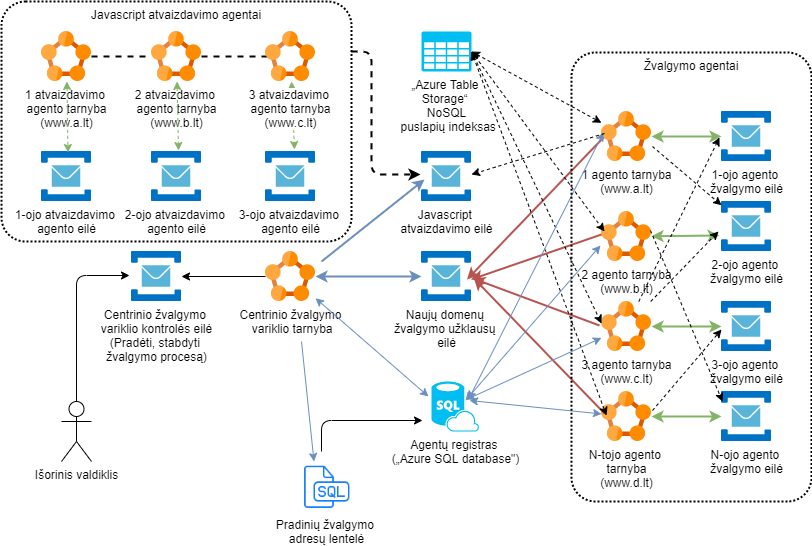
\includegraphics[scale=0.6]{img/Azure_Implementacija_Kasparo.png}
\caption{Struktūrinė prototipo sistemos schema}
\label{fig:azure_implementation_structural_scheme}
\end{figure}

\subsubsection{Duomenų saugojimo talpyklos}

Prototipas naudoja dvi talpyklas agentų informacijai ir puslapių peržiūros būsenai saugoti.

\subsubsubsection{Agentų registras}

„Azure SQL“ duomenų bazė, kurioje apibrėžta:

\begin{itemize}
    \item Peržiūros agentų registracijos lentelė
    \item Javascript atvaizdavimo agentų registracijos lentelė
    \item Pradinis peržiūros URL adresų sąrašas
    \item Javascript klientinio atvaizdavimo karkasų raktažodžių sąrašo lentelė, pagal kuriuos atliekama Javascript atvaizdavimo poreikio indentifikacija
\end{itemize}

 % Table generated by Excel2LaTeX from sheet 'crawling_vs_scraping'
\begin{table}[htbp]
  \centering
  \caption{Agentų registro lentelės schema \cite{MercedCloudBasedWebCrawler}}
    \begin{tabular}{|l|l|l|l|l|}
    \hline
    \textbf{Id} & \textbf{Agento\_Vardas} & \textbf{Agento\_Aptarnavimo\_Sritis} & \textbf{\textcolor{red}{Paskutinis\_Aktyvumas}} & \textbf{Ištrintas} \bigstrut\\
    \hline
    1 & A1 & abc.lt & 2020-05-02 15:30:15 & false \\
    \hline
    2 & A2 & def.lt & 2020-05-02 13:30:15 & true \\
    \hline
    \end{tabular}%
  \label{tab:agent_registry_table}%
\end{table}%
 
 \ref{tab:agent_registry_table} lentelėje pavaizduotame agentų registre raudonai pažymėtas paskutinio aktyvumo laiko stulpelis originaliai \cite{MercedCloudBasedWebCrawler} literatūroje neminėtas, tai -- rašto darbo autoriaus prototipo planavimo metu įgyvendinta korekcija siekiant atlaisvinti nebenaudojamus agentus.
 
 Įgyvendintas algoritmas, atlaisvinantis nebenaudojamus agentus, apibrėžiamas šiais žingsniais:
 
 \begin{enumerate}
     \item Gavus naujo domeno žvalgymo užklausą, centrinis žvalgymo variklis tikrina visų aktyvių agentų paskutinio aktyvumo stulpelio reikšmes
     \item Išrenkami visi agentai, kurių stulpelio „Paskutinis\_Aktyvumas“ reikšmė yra „NULL“ arba < DABARTINIS\_LAIKAS - NUSTATYMUOSE\_APIBRĖŽTAS\_NEAKTYVUMO\_PERIODAS 
     \item Kiekvienam išrinktam agentui tikrinama, ar jo peržiūros eilė yra tuščia, jei taip -- agentas naikinamas ir ištrinama jo peržiūros eilė
 \end{enumerate}
 
 \subsubsubsection{Puslapių indeksas}

Tai -- „Azure NoSQL Table Storage“ duomenų bazė, kurioje saugomi visi surasti URL adresai ir jų peržiūros būsena. \ref{tab:crawling_tablel} lentelėje nurodyta peržiūros URL adresų saugojimo lentelė. \textit{PartitionKey} apibrėžia domeno vardo sritį, o \textit{RowKey} -- MD5 kontroline suma užkoduotas pilnas URL adresas, kuris unikaliai identifikuoja puslapį jo domeno zonoje.

% Table generated by Excel2LaTeX from sheet 'Sheet1'
\noindent \hspace*{4em}%
\begin{table}[ht]
  \centering
  \caption{Peržiūros URL adresų lentelė}
    \begin{tabular}{|l|l|l|l|r|r|r|}
    \hline
    PartitionKey & RowKey & PageUrl & Timestamp & \multicolumn{1}{l|}{Visited} & \multicolumn{1}{l|}{StatusCode} & \multicolumn{1}{l|}{Rendered} \bigstrut\\
    \hline
    abc.lt & 0575118B9D... & abc.lt/naujienos/ & 2020-05-01T...& TRUE & 200 & TRUE \bigstrut\\
    \hline
    def.lt & 52F8F6432... & def.lt/orai & 2020-05-10T... & FALSE &     & FALSE \bigstrut\\
    \hline
    \end{tabular}%
  \label{tab:crawling_tablel}%
\end{table}%


\ref{tab:script_files_tablel} lentelėje pavaizduota skriptų saugojimo informacijos talpykla, kurioje saugomos HTML identifikuotų skriptų kontrolinės sumos ir Javascript atvaizdavimo sprendimas.

\pagebreak

\begin{itemize}
    \item \textit{PartitionKey} -- domeno vardo sritis
    \item \textit{RowKey} -- skripto URL adreso MD5 kontrolinė suma
    \item \textit{Checksum} -- skripto turinio MD5 kontrolinė suma
    \item \textit{ScriptFile} -- skripto pavadinimas
    \item \textit{RenderDecision} -- indikacija, ar rasta klientinio atvaizdavimo požymių
\end{itemize}

% Table generated by Excel2LaTeX from sheet 'Sheet1'
\begin{table}[ht]
  \centering
  \caption{Skriptų informacijos saugojimo lentelė}
    \begin{tabular}{|l|l|l|l|r|}
    \hline
    PartitionKey & RowKey & Checksum & ScriptFile & \multicolumn{1}{l|}{RenderDecision} \bigstrut\\
    \hline
    abc.lt & 0575118B9D... & 3d572837... & bundle.js & TRUE \bigstrut\\
    \hline
    def.lt & 52F8F64324... & 999101d8... & jquery.js & FALSE \bigstrut\\
    \hline
    \end{tabular}%
  \label{tab:script_files_tablel}%
\end{table}%


\subsubsection{Žvalgymo agentai}

Žvalgymo agentai įgyvendinti kaip „Service Fabric“ tarnybos be būsenos (angl. -- \textit{Stateless services}). Kiekvienas iš jų turi savo atitinkamą eilę, iš kurios ima žvalgytinų puslapių URL adresus. Priskirtoje „Service Bus“ eilėje talpinami tik tie puslapių URL adresai, kurie priklauso agentui priskirtai domeno vardo sričiai.

\subsubsection{Centrinis žvalgymo variklis}

Šis komponentas taip pat įgyvendintas, kaip „Service Fabric“ tarnyba be būsenos, jis sukuriamas iš karto paleidus klasterį ir yra atsakingas už naujų agentų ir jų žvalgymo eilių kūrimą/naikinimą. Šis komponentas klausosi 3 skirtingų „Service Bus“ eilių ir apdoroją jų žinutes:

\begin{itemize}
    \item \textbf{Centrinio žvalgymo variklio kontrolės eilė} -- į šią eilę roboto klientinė sąsaja talpina peržiūros komandas: pradėti, stabdyti peržiūros procesą, keisti aktyvių agentų skaičių
    \item \textbf{Naujų domenų žvalgymo užklausų eilė} -- tai pagrindinė „žvalgymo pasienio“ eilė, kurioje kaupiami visi URL adresai neturintys aktyvaus peržiūros agento. Jeigu agentas visgi egzistuoja, žvalgymo variklis atvykusį URL adresą peradresuoja jo atitinkamai žvalgymo eilei. Kitu atveju, žvalgymo variklis bando URL adresui kurti naują agentą, jei neviršytas maksimalus aktyvių agentų limitas
    \item \textbf{Javascript atvaizdavimo eilė} -- šioje eilėje talpinami URL adresai tų puslapių, kuriems buvo nustatyta indikacija, jog jie naudoja klientinį Javascript atvaizdavimo karkasą. Centrinis žvalgymo variklis gavęs žinutę iš šios eilės, patikrina, ar maksimalus aktyvių Javascript atvaizdavimo agentų skaičius neviršytas ir bando kurti atvaizdavimo agentą URL adreso domeno vardo sričiai.
\end{itemize}

\subsubsection{Javascript atvaizdavimo agentai}

Šių agentų veikimo principas beveik identiškas žvalgymo agentams -- jie turi savo domeno srities atvaizdavimo eiles. Skirtumas, jog pastarieji nenaudoja paprastų HTTP užklausų į URL adresu pasiekiamą žiniatinklio serverį, o pasitelkia kitoje „Service Fabric“ tarnyboje esančią „Chromium“ tvarkyklę, kuri turi integruotą Javascript atvaizdavimo variklį. Javascript atvaizdavimo agentai su šia tarnyba bendrauja per „Websocket“ protokolo jungtį, kuri leidžia tinklu kontroliuoti nutolusią naršyklę, tereikia paleidžiant tvarkyklę nurodyti parametrą, apibrėžiantį prisijungimo jungtį: \textit{chrome.exe --remote-debugging-port=9222}.

\subsection{Kiti prototipo realizacijoje panaudoti įrankiai}

Šiame poskyryje aprašomos įgyvendinant prototipą panaudotos bibliotekos, vykdomosios aplinkos, programavimo kalbos.

\subsubsection{Programavimo aplinka}

„Service Fabric“ klasterio kodas buvo rašytas C\# programavimo kalba panaudojant .NET Core 3.1 karkaso, kuris leidžia vienai kodo bazei veikti skirtingose operacinėse sistemose, versiją. Daug panaudotų „NuGet“ paketų valdymo sistemos bibliotekų (pvz.: PuppeteerSharp, AngleSharp) palaiko .NET Standard 2.0 versiją, kuri skirta tiek tradiciniam .NET karkasui, tiek ir .NET Core aplinkai.

\subsubsection{Bibliotekos}

\begin{itemize}
    \item \textit{AbotCrawler}\footnote{Abot -- https://github.com/sjdirect/abot} -- patogi ir aktyviai palaikoma .NET biblioteka, skirta specialiai puslapių žvalgymui. Įgyvendina daug žemo lygio funkcinių žvalgymo detalių (DNS išaiškinimas, žvalgymo intervalai, etiško žvalgymo politiką), todėl programuotojas gali papildomai nebesirūpinti jų įgyvendinimu
    \item \textit{Dapper} -- minimali ORM biblioteka, skirta komunikacijai su duomenų baze. Prototipui nereikėjo ORM bibliotekų, tokių kaip Entity Framework, funkcionalumo, todėl įgyvendinant achitektūrinį repozitorijos sluoksnį panaudotas šis paketas, kuris reikalauja rašyti užklausas rankomis \cite{DapperORM}
     \item \textit{AngleSharp} -- HTML dokumento apdorojimo .NET biblioteka, leidžianti serverio pusėje sukurti DOM medį, jį analizuoti, išgauti informaciją, keisti \cite{AngleSharp}. Panaudota Javascript skriptų išgavimui.
      \item \textit{PuppeteerSharp} -- komunikacijai su „Chromium“ tvarkykle naudojama .NET biblioteka, kuri originaliai sukurta Node.JS platformai \cite{PuppeteerSharp}. Ši biblioteka naudojama Javascript atvaizdavimo agentų prisijungimui „Websocket“ jungtimi prie „Chromium“ tvarkyklės agento
\end{itemize}

\subsection{Panaudojamumo atvejų dinamika}

Šiame poskyryje detaliau grafiškai pristatomos apibrėžtų panaudojamumo atvejų algoritminės sekos, kurios perteikiamos UML sekų diagramomis. 

\subsubsection{U1.1 Inicijuoti peržvalgos procesą}

Žemiau pateiktoje \ref{fig:initiate_crawling_uml_sequence} UML sekos diagramoje pavaizduotas sistemos administratoriaus inicijuojamas žvalgymo pradėjimo procesas, kurio metu pradinis URL adresų sąrašas perkeliamas į žvalgymo pasienio komponentą ir sukuriamas pradinis žvalgymo agentas.
\begin{figure}[ht!]
\centering
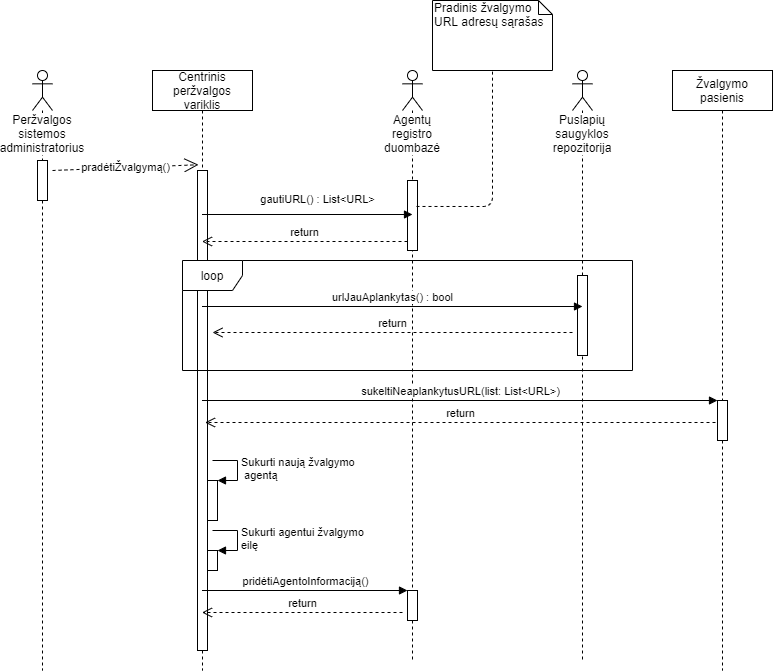
\includegraphics[scale=0.6]{img/initiate_crawling_process_sequence.png}
\caption{Žvalgymo inicijavimo proceso UML sekos diagrama}
\label{fig:initiate_crawling_uml_sequence}
\end{figure}

Peržvalgos sistemos administratorius yra klientinė programa, valdanti robotą. Galima realizuoti tiek žiniatinklio, tiek darbalaukinės programos klientą. Prototipo realizacijos metu klientas simuliuojamas naudojant „Service Bus Explorer“ eilių programą ir rankomis siunčiant žinutes į valdymo eilę.

\pagebreak

\subsubsection{U2 Vykdyti puslapio peržvalgą}

\ref{fig:perform_crawling_uml_sequence} UML sekos diagramoje pavaizduota žvalgymo agento darbo vykdymo schema. Akcentuotina, kad šis žvalgymo procesas kartojamas iki to laiko, kai žvalgymo agento eilė tampa tuščia ir po sistemos konfigūracijoje nustatyto agento neaktyvumo intervalo, Centrinis žvalgymo variklis tiesiog panaikina nebeaktyvų žvalgymo agentą.

\begin{figure}[ht!]
\hspace*{-2cm} 
\centering
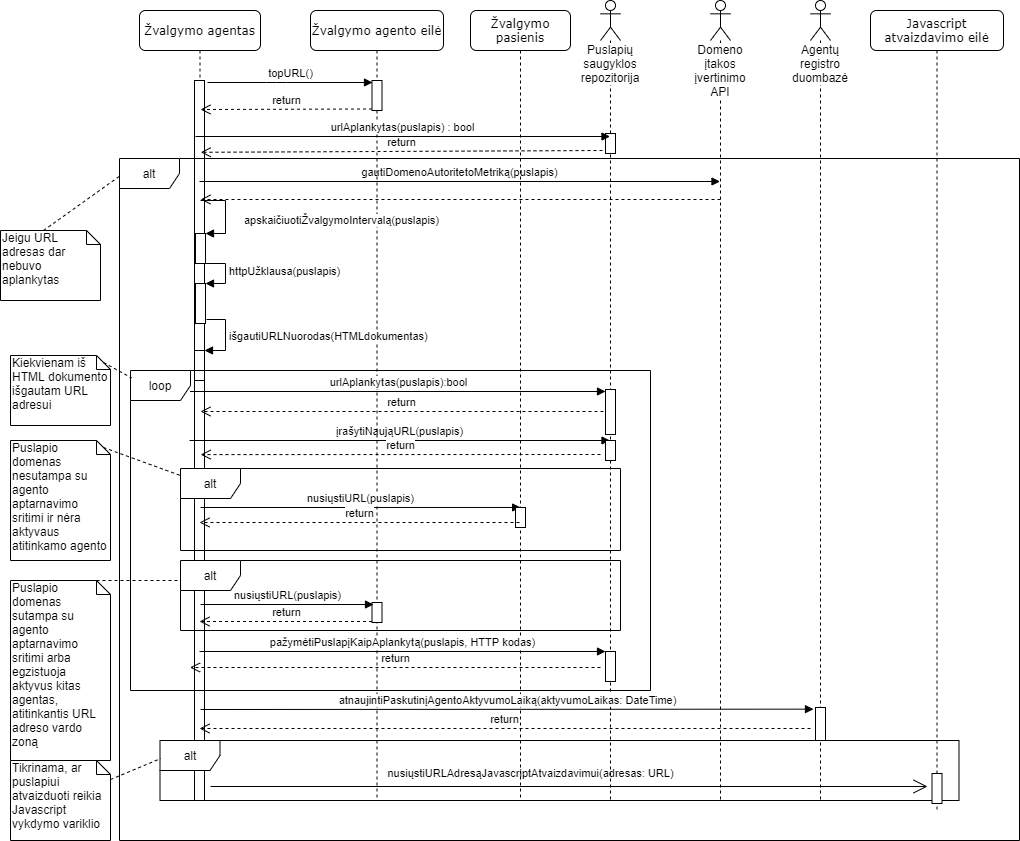
\includegraphics[scale=0.5]{img/perform_cralwing_sequence.png}
\caption{Žvalgymo vykdymo proceso UML sekos diagrama}
\label{fig:perform_crawling_uml_sequence}
\end{figure}

\subsubsection{U2.1 Įvertinti, ar puslapis vykdo klientinį Javascript atvaizdavimą}

\ref{fig:perform_crawling_uml_sequence} diagramoje paminėta, jog URL adresas po žvalgymo į Javascript atvaizdavimo eilę siunčiamas tik nustačius, jog puslapis reikalauja Javascript atvaizdavimo variklio, kad galėtų dinamiškai generuoti DOM medį. Šiame punkte pateikiama UML veiklos diagrama \ref{fig:js_rendering_condition}, kurioje nurodoma, kaip prototipinė sistema atlieka šį tikrinimą.

\begin{figure}[ht!]
\centering
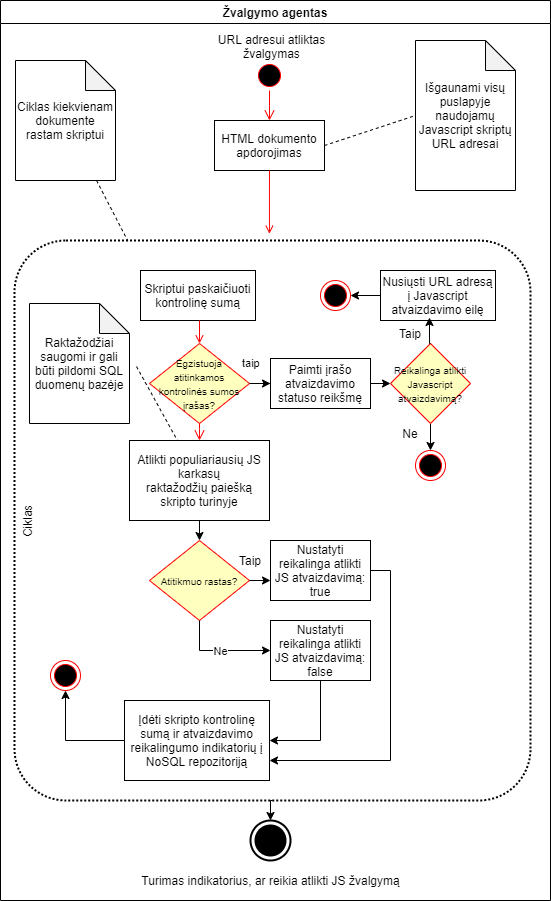
\includegraphics[scale=0.6]{img/javascript_rendering_condition_activity_diagram.png}
\caption{Poreikio atlikti Javascript atvaizdavimą indikatoriaus nustatymo UML veiklos diagrama}
\label{fig:js_rendering_condition}
\end{figure}

Šiame skyriuje aprašytos architektūros prototipo peržiūros greitaveika išbandoma eksperimentinio tyrimo, aprašyto 7 skyriuje, metu.
\section{Eksperimentinis prototipo vertinimas}
\subsection{Sistemos tyrimo sąlygos}
\subsection{Greitaveikos tyrimo rezultatai}
\subsection{Sistemos komponentų veikimo stebėjimo rezultatai}
\subsection{Viešai prieinamų sistemų eksperimentinis vertinimas}
\sectionnonum{Rezultatai}

Darbe pasiekti \textbf{rezultatai}: 

\begin{enumerate}
    \item Atlikta saityno peržiūros robotų probleminės srities literatūrinė apžvalga: 
    \begin{itemize}
        \item identifikuoti saityno nuorodų ryšiai remiantis grafų teorijos sąvokomis
        \item pristatytas bazinis peržiūros robotų veikimo algoritmas
        \item atliktas saityno peržiūros robotų ir saityno duomenų surinkimo robotų sistemų palyginimas: išskirti panašumai ir trūkumai
        \item aprašytos 3 saityno peržiūros robotų veikimo politikos: \textbf{pasirinkimo}, \textbf{etiško žvalgymo} ir \textbf{pakartotinio apsilankymo}
        \item Identifikuotos 4 peržiūros robotų kategorijos: \textbf{plačiosios peržiūros}, \textbf{teminės peržiūros}, \textbf{inkrementinės peržiūros}, \textbf{išskirstytos peržiūros}
    \end{itemize}
    
    \item Apibrėžti saityno peržiūros robotų komponentai ir jų paskirtis: \textbf{peržiūros pasienis}, \textbf{HTTP parsiuntimo modulis}, \textbf{saityno nuorodų ištraukiklis}, \textbf{adresų skirstiklis} , \textbf{adresų filtras}, \textbf{dublikatų šalintojas}, \textbf{adresų prioritizuotojas}. Remiantis identifikuotais komponentais, UML veiklos diagrama apibrėžtas saityno peržiūros vykdymo ciklas
    
    
    \item Palygintos 3 saityno peržiūros robotų architektūros analizuojant peržiūros išplečiamumo ir darbo koordinavimo aspektus: \textbf{„PolyBot}, \textbf{„Mercator“}, \textbf{„Heritrix“} 
    
    
    \item Palygintas \textbf{tradicinis} ir \textbf{AJAX žiniatinklio atvaizdavimo} modeliai, identifikuotas saityno peržiūros robotų ribotumas žvalgyti AJAX tipo svetaines, pristatytas „Googlebot“ peržiūros roboto taikomas modelis atvaizduojant dinaminį turinį generuojančias svetaines
    
    
    \item Apibrėžta 12 funkcinių ir 3 nefunkciniai saityno peržiūros roboto prototipo reikalavimai
    
    
    \item Pristatytos prototipo įgyvendinumui pasirinktos „Azure“ debesų kompiuterijos tiekėjo technologijos: \textbf{„Service Fabric“ orchestravimo platofrma}, \textbf{„Service Bus“ eilių infrastruktūra}, \textbf{„Azure Table Storage NoSQL saugykla“}, \textbf{„Azure SQL“ duomenų bazė}. Argumentuoti pasirinkimo motyvai, identifikuotos nepasirinktos alternatyvos
    
    \item Įgyvendintas saityno peržiūros roboto prototipas:
    \begin{itemize}
        \item Apibrėžti 7 panaudojamumo atvejai, kurie atsekamumo matrica susieti su prototipui iškeltais reikalavimais
        \item Pristatyta realizuojant prototipą naudojama architektūra
        \item Nubrėžtos prototipo dinamiką vaizduojančios UML sekų ir veiklos diagramos, taip pat struktūrinė schema
        \item C\# kalba, naudojant .NET Core karkasą realizuotas apibrėžtos architektūros prototipas, aprašytos panaudotos bibliotekos
    \end{itemize}
    
    
    \item Atliktas prototipo vertinimas -- įvykdytas roboto veikimo stebėsenos eksperimentas, surinktos ir išanalizuotos funkcinės metrikos, taip pat prototipo komponentų apkrovos
\end{enumerate}
\sectionnonum{Išvados}
\sectionnonum{Galimos ateities darbų kryptys}

\printbibliography[heading=bibintoc]
 
% \appendix
% \input{annexes/attributeStoreContract}
% \input{annexes/serviceRegisterContract}
% \input{annexes/appSketches}

\end{document}
